\usepackage{hyperref}
\usepackage{hyperref}

% Colors
\definecolor{colorCellHighlight}{rgb}{0.85, 0.91, 0.97} % You can define Your own colors this way


% References
% Here You can choose the reference style

% ACM-style. Numeric references [1]. Alphabetical order.
% \usepackage[style=unitartucs/citations/numeric]{biblatex}

% IEEE-style. Numeric references [1]. Reference order.
\usepackage[style=unitartucs/citations/numeric,sorting=none]{biblatex}

% AMS-style. Trigraph references [ABC]. Alphabetical order.
% \usepackage[style=unitartucs/citations/alphabetic]{biblatex}

% APA-style. References with name and year (Koit 2010). Alphabetical order.
% \usepackage[style=unitartucs/citations/authoryear,uniquename=init]{biblatex}

\addbibresource{english/references.bib} % This file contains your bibliography entries


% Metadata
\title{Eyes Wide Shut: Analyzing Object Detection Performance under Degraded Sensor Input Scenarios.}
\author{Author's Name}
\date{2024}
\supervisor{Supervisor's Name\degree{degree} \and Co-Supervisor's name\degree{degree}}
\curriculum{Computer Science Curriculum}
\thesis{Bachelor's Thesis (9 ECTS)}
\keywords{Layout, formatting, template}


% Here begins the document

\begin{document}

\maketitle

\linespread{1.45} \selectfont

\newpage
\pdfbookmark[1]{\infoname}{info} % Lisame infolehe PDF-faili järjehoidjatesse.

% Eesti keeles info.
\begin{infoEst}
\begin{abstract}
Siia kirjutage oma lõputöö lühikokkuvõte. See võib lühidalt teemasse sisse juhatada, kuid peaks enamikus katma ära Teie lõputöö sisu. Seda lugedes peaks olema üheselt selge, millest Teie lõputöös lugeda võib. Hea on näiteks kirjutada eesmärgi, meetodi, tulemuste ja järelduste kohta. Bakalaureusetöö korral võiksid nii eesti kui inglise keeles olevad lühikokkuvõtted mahtuda ühele leheküljele. Magistritöö või vajaduse korral võib eesti ja inglise keeles olevad osad kirjutada eraldi lehekülgedele. Mõelge oma tööd kirjeldavad võtmesõnad ning leidke CERCS kood(id).
\end{abstract}

\keywords{\@keywords}
\cercs{KOOD Koodi nimi}

% Koodid leiate: https://www.etis.ee/Portal/Classifiers/Index/26
% Nt: P170 Arvutiteadus, arvutusmeetodid, süsteemid, juhtimine (automaatjuhtimisteooria)
% Nt: P175 Informaatika, süsteemiteooria

\end{infoEst}


% Inglise keeles info.
\begin{infoEng}
\begin{abstract}
Write here the abstract of your work. The abstract could provide a brief introduction to the topic but should, in the majority, cover Your thesis work. When reading the abstract, it should become clear what can be read about in the rest of Your thesis. It is good to write about the purpose of the thesis, method(s), results, and findings of Your work. For a bachelor’s thesis, both the Estonian and English abstracts should fit into a single page. For a master’s thesis or when necessary, the Estonian and English sections of this page could be on separate pages. Come up with good keywords for Your work and find your CERCs code(s).
\end{abstract}

\keywords{Layout, formatting, template}
\cercs{CODE Code name in English}

\end{infoEng}

\newpage
% \newpage
\pdfbookmark[1]{Visual Abstract}{visualsummary} % Adding the file to PDF bookmarks
\section*{Visual Abstract}

\begin{figure}[ht]
    \centering
    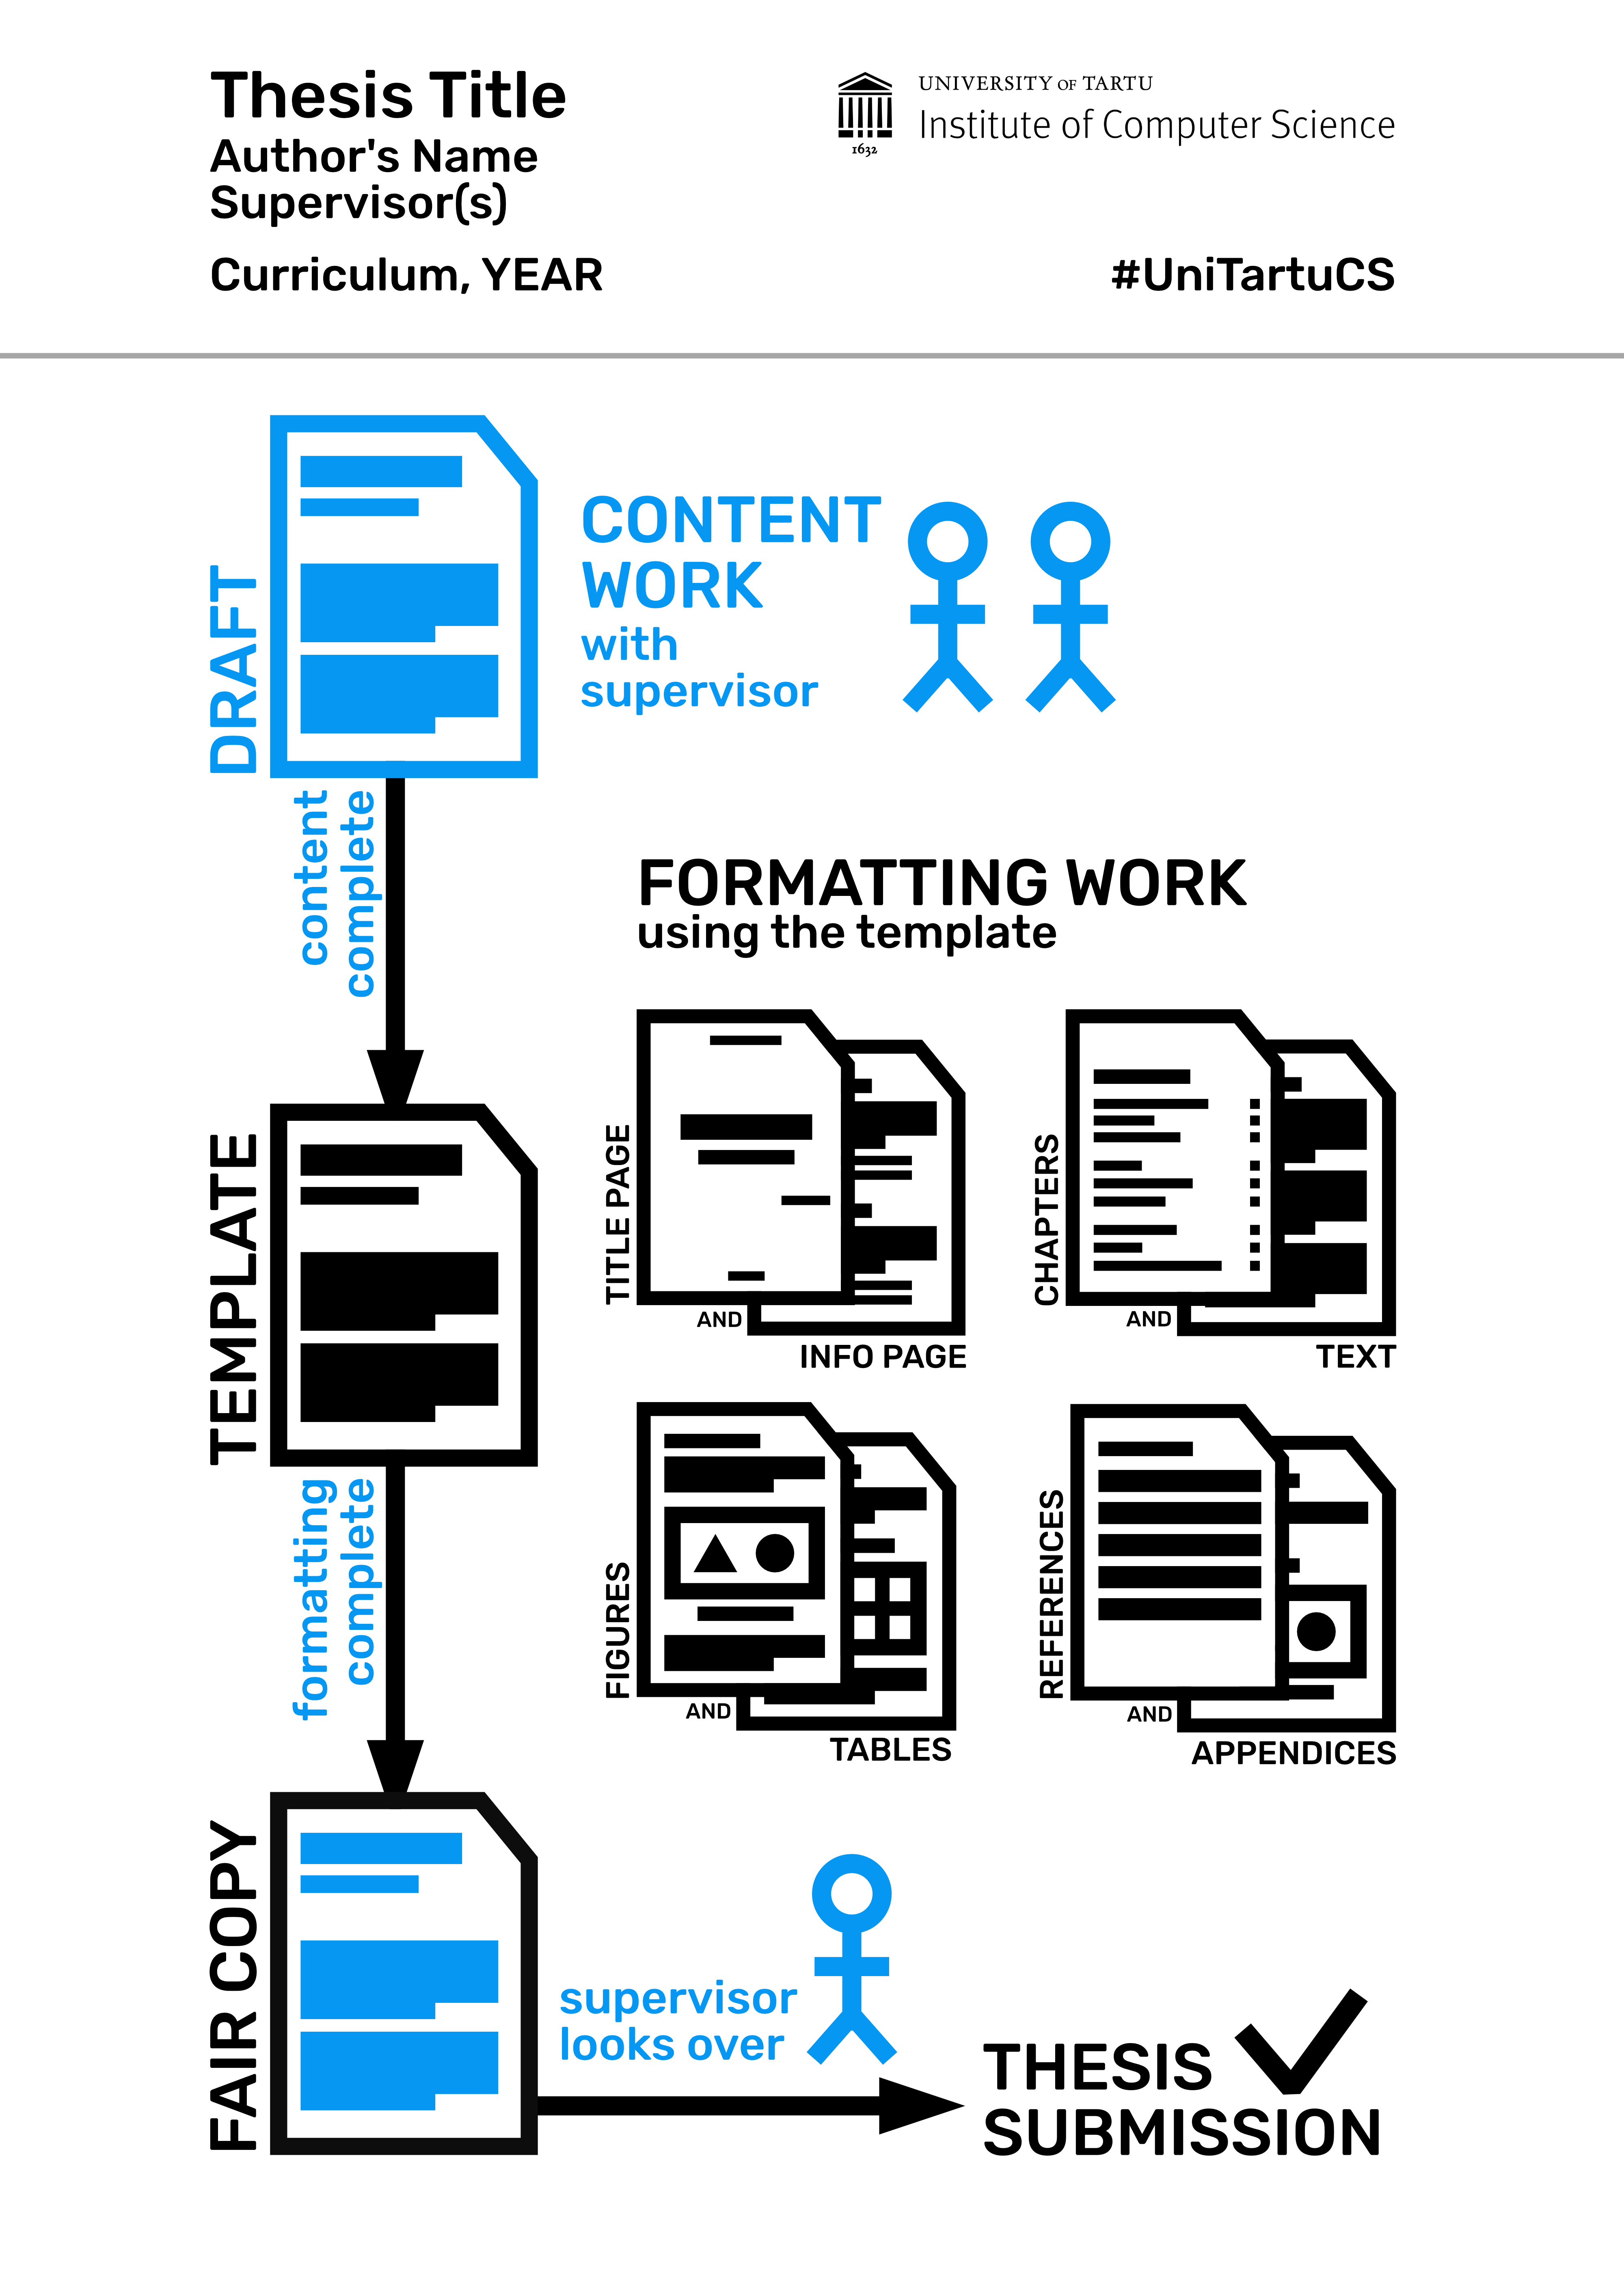
\includegraphics[width=0.85\textwidth]{figures/Figure0-VisualAbstract.png}
    \label{fig:visual-abstract}
\end{figure}

\newpage


\tableofcontents

\section{Introduction} \label{Introduction}

% Justification for the choice of topic
Autonomous driving systems promise to revolutionize transportation by increasing road safety, improving traffic efficiency, and reducing emissions \cite{litmanAutonomousVehicleImplementationb}.
% actuality
Autonomous driving systems are complex systems equipped with multi-sensor perception, integrating data from various sources. Autonomous driving systems should be capable of operating in various environments under diverse weather conditions. Autonomous vehicles are not yet ready, and mistakes or technical failures can cause accidents and undermine public trust.

% novelty
Autonomous driving systems heavily rely on deep learning for multiple perception tasks. Object detection is foundational among these tasks. In spite of the significant progress in this area, there is still a need for an effective and efficient general model architecture that is capable of understanding input from multiple sensors and is robust.

% Overview Theoretical Background -- background information to contextualize the problem
% review of state of the art solutions

Simple still-image detectors \cite{} cannot be applied to video data, because it contains challanges such as motion blur, occlusion etc.. Another approaches \cite{hanSeqNMSVideoObject2016, kangTCNNTubeletsConvolutional2018, kangObjectDetectionVideo2016} integrate a postprocessing after object detection improve results but those solutions are not end-to-end solutoins.

Another line of approaches \cite{Lu_2017_ICCV, xiaoVideoObjectDetection2018} leverages a second model to integrate motion and temporal information during training. 


% Problem statement -- if necessary, it should include the posed hypothesis/hypotheses, research questions, and subject of research

All of those detection pipelines for video object detection are over sophisticated, requiring many hand-crafted components, not capable of handling other modalities than images.

% Purpose of the Thesis -- overall aim and objective of the research, "why" of the research—why are you conducting this study?

In this thesis, our goal is to present a noval recurrent architecute we call Recurrent Perceiver inspired by Perceiver arhitecture. We present a training framework to asses robastness of the model.
Our main contributions are as follows:

\begin{itemize}
\item We propose a Recurrent Perceiver architecture. By unrolling it in time, the model can be interpreted as a recurrent neural network (RNN). Furthermore, the model supports multiple sensory inputs.
\item We propose a task to predict object center points and introduce custom-created benchmarks, which we call "detection-moving-mnist-easy," for evaluating this task.
\item We designed an experiment to simulate degraded input scenarios for single or multi-sensor (camera) setups. We evaluate the proposed Recurrent Perceiver, demonstrating that our training procedure with omitted input consistently achieves improved performance compared to training without dropout.
\end{itemize}

% [//]: # (The description of the structure of the thesis by chapter)

% A brief section giving background information may be necessary, especially if your work spans two or more traditional fields. That means that your readers may not have any experience with some of the material needed to follow your thesis, so you need to give it to them. A different title than that given above is usually better; e.g., "A Brief Review of Frammis Algebra.

Section~\ref{Background} gives background information about autonomous driving system architecture and overviews relevant video object detection approaches, and introduces original Perceiver model achitecture. Section~\ref{Methods} presents a noval Recurrent Perceiver architecture, presents benchmark used for training and testing, and explains training procedure. Section~\ref{Experiments} explains experiments and presents results.




% a short overview of appendices including the content of attached materials
% TODO

% TODO: Question where should i put it?
% This thesis was written using the Overleaf1 text editor. The text was checked with the
% Grammarly2 writing assistant to catch typos and other grammatical errors.
% \section{Formatting}  \label{formatting}
Many different tools, some of which You might not even be aware of, will be used to format Your thesis. As good formatting makes up 25\% of Your thesis grade, it is important to take it seriously and allocate sufficient time. Especially if You have not previously formatted documents of that size that well or learned the use of corresponding tools. This chapter looks at the formatting principles for different parts of the thesis.

\subsection{The Title and Info Pages}
The very first page – the title page – is already formatted in this template. The title page must include the curriculum You plan to graduate from (including the educational institution and the institute), thesis title, kind and volume corresponding to the level of studies, Your name, the names (and, optionally, the academic degrees) of Your supervisors, publication location, and year. The information that goes to your title page must be entered into the specific fields in the file \path{thesis.tex}. Be sure to check the corresponding information. For example, if You decide to add the academic degrees of Your supervisors, check if an abbreviation is MSc (Master of Science) or MA (Master of Arts). The degrees differ depending on the curricula.

The info page (file \path{0-info.tex}), which follows Your title page, includes the abstract, keywords, and CERCS codes of Your work. The abstract should give an overview of everything done during Your work. For example, if three of Your content chapters thoroughly describe the different processes and results of Your work, then that should be readable from Your abstract. Concentrate on mentioning in the abstract what You did that can be read about in the thesis.

Keywords are the different terms and names that designate important aspects of Your work. To come up with keywords, You should think about Your work generally. What important terms come to Your mind if You think about Your work as a whole? For inspiration, it is good to check out the keywords of previous theses made on similar topics. Joonis~\ref{fig:keywords} shows the word cloud of keywords from the theses defended at the Institute of Computer Science in 2015–2020\footnote{\url{https://cglearn.eu/theses/top}}.

\begin{figure}[ht]
    \centering
    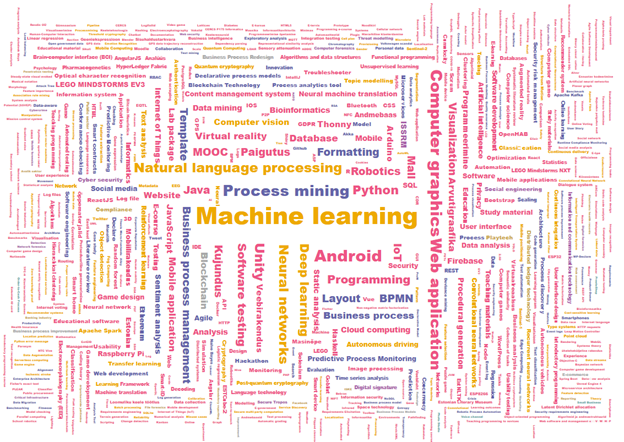
\includegraphics[width=\textwidth]{figures/Figure1-Keywords.png}
    \caption{The word cloud of keywords from theses defended at the Institute of Computer Science in 2015–2020.}
    \label{fig:keywords}
\end{figure}

Besides the keywords, You also need to assign a Common European Research Classification Scheme (CERCS) code to Your work. These codes classify research areas. Often, it can be hard to classify a thesis using a specific classifier. Still, You must find a classifier that Your work fits under the best. You can use several CERCS codes. The classifiers are on the Estonian Research Information System’s web page: \url{https://www.etis.ee/Portal/Classifiers/Index/26}.

After the info page, You can also add a visual abstract to Your work. That will be a single figure that efficiently describes the process and results of Your work. The figure has to include the information listed in the Guidelines for preparing and grading of graduation theses at the Institute of Computer Science of the University of Tartu document. When using the institute’s logo, respect its protected area – it must have the height of the house of free space around it. The visual abstract is helpful to add, as it quickly conveys the nature of Your work to the reader. You can reuse the graphics later on Your defense slides and when popularizing Your work.

\subsection{Structure}
It is essential for the reader of Your work that Your document is structured logically and clearly. Good titles and reasonable content sectioning to chapters and sub-chapters guide the reader through Your thesis.

\subsubsection{Titles}
Both the thesis title itself and the chapter titles should be concise and on-point. Long titles could carry too many ideas within themselves, and You can lose Your reader already at the title. The main title of the thesis should maximally fit on two lines.

In English, the words in titles start with capital letters. There are different styles, but generally, all the words besides pronouns should start with a capital letter. It is good to use the Capitalize My Title tool: \url{https://capitalizemytitle.com/}

In Estonian, however, only the very first letter of the title is capitalized, and the rest of the words are written just like regularly.

Punctuation should be avoided in titles. Depending on the nature of Your work, an em or en dash could be reasonable. For example, if You have created a software product, it is good to mention the product's name in the title, followed by a longer dash and a description of its unique value. On the other hand, a sentence with commas or question marks would not fit as a title.

These principles also apply to the titles of Your chapters, which are called headings. The content chapter headings start with numbers. It is up to You if You start the numbering from the Introduction chapter and end it with the Conclusion chapter or leave these two chapters unnumbered. In this template, the Introduction and Conclusion chapters are also numbered. The Conclusion chapter is followed by unnumbered sections called References and Appendices. For different appendices, it is reasonable to use some numbering again. To number the appendices, You can use Roman numerals (Appendix I, Appendix II) or capital letters (Appendix A, Appendix B).

The subchapter numbering includes the number from the parent chapter. For example, the subchapters of chapter 2 are numbered 2.1, 2.2, etc. The dot mark after the entire numbering is used only in the first-level headings. Starting from the third-level headings, the numbering can be omitted. In this template, the heading styles (\verb|\section{...}|, \verb|\subsection{...}|, etc) provide the correct numbering.

\subsubsection{Table of Contents}
At the beginning of Your work, after the info page and visual summary, but before the first chapter, there is the Table of Contents. Capable text editing software generates the Table of Contents automatically. In this template, the table of contents is created by the command \verb|\tableofcontents|. That command generates the table of contents automatically based on the sections/headings (\verb|\section{...}|, \verb|\subsection{...}| jne) of the document.

\subsection{Text}
The alignment of the thesis text must be justified (straight rug from both left and right). Justified alignment can create a situation when the spacing between words in one line is visually too much. In such cases, the line can be hyphenated to fix the visually bothersome spacing. Many text editors have automatic hyphenation capabilities, but these are prone to over-hyphenation. In this template, the automatic hyphenation is minimized and the package \verb|microtype| ensures that the spacing between the words would not get too large. Having hyphenated words hinders the readability of the text, so hyphenation should be used minimally. One should avoid situations when multiple subsequent rows are hyphenated.

The guidelines for preparing and grading of graduation theses at the Institute of Computer Science of the University of Tartu document presents many text formatting rules. For example, the line spacing of text should be in the range 1.0-1.5. This template uses 1.4 line spacing which visually corresponds to the 1.5 line spacing of Microsoft Word.

It is possible to use italics (\verb|\emph{...}|), bold (\verb|\textbf{...}|), or other text formatting tools to emphasize some terms or ideas in Your text. However, it is good to use these tools sparingly so as not to make Your work visually too hectic.

When writing paragraphs, You should observe that there would not be a single lone word at the last row of the paragraph. This is called an orphan word, and it is not visually very good. Checking for orphan words or lines (an orphaned line of text at the beginning of a page that is followed by a new chapter or empty page) is something one should do as one of the last things when formatting their fair copy.

\subsection{Elements}
Many different elements like figures, tables, and code examples improve the appearance and reader’s understanding of Your thesis.

\subsubsection{Figures}
All the different images, be they plots, photographs, or screenshots, are labeled as figures. When adding an image, it should be labeled as a figure, numbered, and captioned. In the LaTeX template here, this is done by first adding or uploading the image to the \verb|figures| folder. Afterward the image can be used via the following code:

\begin{minted}[escapeinside=||]{tex}
\begin{figure}
    \centering
    \includegraphics[width=\textwidth]{figures/|\textbf{Figure1-Name.png}|}
    \caption{|\textbf{Figure caption text.}|}
    \label{fig:|\textbf{figureLabel}|}
\end{figure}
\end{minted}

The code above must include the correct file name with the file extension inside the \verb|figures| folder, a short caption text, and a short \emph{label} for cross-referencing the figure.

It should be clear from the caption what is depicted in the image. The caption is shown under the figure together with the element's label \emph{Figure} and an automatic number.

\begin{wrapfigure}{r}{0.33\textwidth}
    \centering
    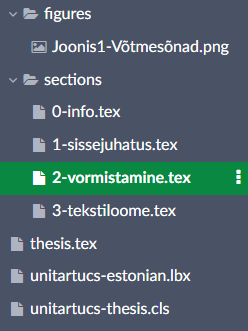
\includegraphics[width=0.33\textwidth]{figures/Figure2-figuresFolder.png}
    \caption{Template folders.}
    \label{fig:folders}
\end{wrapfigure}

You can add the images in the middle of the page or wrap text around them. To add a figure that is wrapped by text, write \verb|wrapfigure| instead of \verb|figure| in the example above. The figure's width could be, for example, \verb|width=0.33\textwidth|.

It is recommended to wrap the text around the image in situations where the image is about 1/3 of the width of the page. In other situations, it is likely better to have the image in the middle of the page without text wrapping.

When positioning the images, You have to be very careful not to scale the image unevenly. Both the vertical and horizontal scale of the image must change the same proportion. Typically this issue does not happen in LaTeX, but you should still consider it when working on the figures with other software.


We recommend creating a solid color palette when creating images. This means that You use the same colors (or course with the same semantics) for plots throughout Your thesis. A useful tool for creating a color palette is Coolors: \url{https://coolors.co/generate}. Depending on the situation, You need to consider that the chosen colors support the readability of Your plots. For example, You should not pick two very similar colors to represent different data points. Tamara Munzner has presented principles about data visualization in her talk Keynote on Visualization Principles~\cite{tamara_munzner_keynote_2012}. A good and cohesive color palette and style are crucial not only for plots but also for graphical elements added to screenshots or for figures in general.

\subsubsection{Tables}
A thesis can also include tables, in addition to figures. When adding tables, You should consider that reading very large tables is difficult and perhaps the data within them should rather be visualized on a plot. However, sometimes, it is important to represent the data as a table. Smaller tables can fit very nicely into the contents of a thesis. Larger tables can be added in the appendices (either in the Appendices section or as a file in the Accompanying Files archive).

The recommendations for figures are also the same for tables. The only difference is that the caption of a table goes above the table (the caption of a figure was below). For example, look at Table~\ref{tabel:elementDifferences}.

\begin{table}[htb!]
    \centering
    \caption{The differences between formatting figures and tables.}
    \label{tabel:elementDifferences}
    \begin{tblr}{width=1.0\textwidth, hlines, vlines,
                    colspec = { Q[r,font=\bfseries] Q[c] X[c] },
                    row{1} = {font=\bfseries},
                    cell{3}{2} = {bg = colorCellHighlight},
                }
                & Caption Placement     &   Content        \\
    Figure      & Below                 &   Images, graphs, photographs, screenshots     \\
    Table       & Above                 &    Data       \\
    Code Example& Below or absent       &    Program code, psudocode       \\
    \end{tblr}
\end{table}

The table \ref{tabel:elementDifferences} above is created with the following code:
\begin{minted}{tex}
\begin{table}[htb!]
    \centering
    \caption{The differences between formatting figures and tables.}
    \label{tabel:elementDifferences}
    \begin{tblr}{width=1.0\textwidth, hlines, vlines,
                    colspec = { Q[r,font=\bfseries] Q[c] X[c] },
                    row{1} = {font=\bfseries},
                    cell{3}{2} = {bg = colorCellHighlight},
                }
            & Caption Placement & Content                             \\
    Figure  & Below             & Images, graphs, photos, screenshots \\
    Table   & Above             & Data                                \\
    Code    & Below or absent   & Program code, psudocode             \\
    \end{tblr}
\end{table}
\end{minted}

That code is similar to the code for figures from before but has two environments. First, there is the \verb|table| environment which includes the caption preceeding the table. Then comes the \verb|tblr| environment that includes the table itself. In this case, the width of the table is the full width of the page \verb|1.0\textwidth| and the table has all the borders with \verb|hlines| and \verb|vlines|. The cells are created such that the first two are tight (\verb|Q|) and the last one has all the leftover space (\verb|X|). The cells are aligned such that the first one is right-aligned \verb|r| and the other ones center-aligned \verb|c|. The first column and row are written in bold and the cell with index (3,2) is colored light blue.

\subsubsection{Code}
When You bring examples of program code, You should use a monospace font. You should pick one and use it cohesively throughout Your thesis text. Examples of these are Consolas and \texttt{Courier New}. This template uses the \verb|fontspace| package that has the \texttt{Courier New} font\footnote{\url{https://www.overleaf.com/learn/latex/Questions/Which_OTF_or_TTF_fonts_are_supported_via_fontspec\%3F}}.

The formatting of code examples is not as regulated as figures and tables. Brief code examples can be written inside paragraphs. For example, one can write that declaring a variable and assigning a value can be done with code \verb|var a = 10;|. For longer code examples, You should create a separate block like this:

\begin{minted}{javascript}
function add(a, b) {
    return a + b;
}
\end{minted}

The example above uses the \verb|minted| environment from the \verb|minted| package. That environment is configured to add a border around the paragraph containing the code example and uses a monotype font. The \verb|minted| environment can also color the code of certain programming languages to make the code more readable\footnote{\url{https://www.overleaf.com/learn/latex/Code_Highlighting_with_minted\#Reference_guide}}. The text surrounding the code block must address the code example in a sufficiently clear and helpful manner.

\subsubsection{Mathematical Equations}
Formatting mathematical equations is relatively easy in LaTeX. To write a short equation inside regular text, the equation must be surrounded with \verb|$|-signs. For example, an equation descirbing addition is $a+b=c$. For a larger equation, the equation must be added inside the \verb|equation| environment.
\begin{equation}
    \frac{a + b}{c} = d
    \label{eq:abcd}
\end{equation}

The example above is created with the following code:
\begin{minted}{tex}
\begin{equation}
    \frac{a + b}{c} = d
    \label{eq:abcd}
\end{equation}
\end{minted}

As seen, an equation can also have a short label, it gets an automatic number and the label can be used to reference the equation from the text. For example, the example above in this template has a number ~\ref{eq:abcd}.

\subsection{References}
Correctly citing Your sources is very important in Your work. Failure to do so may result in academic fraud, which can cause Your thesis to get a negative review. This template explores three types of references. These are the cross-references between the different elements of the thesis, the footnote references for the so-called weak external references, and the main references, which are also called strong references.

\subsubsection{Ristviited}
All the figures, tables, and mathematical equations must be cross-referenced from the text. The purpose of that rule is to ensure that the illustrative elements actually support Your content.  The added element must be connected with Your text and cross-referenced in a suitable place. The element you cross-reference must have a label and to that label a cross-reference can be created with the command \verb|\ref{label}|. The reference will be a number that turns into a link inside the text (that remains when exporting a PDF). This means that the reader is taken to the referenced element when they click on the cross-reference.

\subsubsection{Footnote References}
The external references can be called as weak and strong. This does not mean anything about their influence or usefulness to Your work. For some external sources, You must make a subjective decision if the reference will be rather the so-called weak or strong one. Weak references are, for example, references to Wikipedia pages, Stack Overflow posts, webpages of products, dictionaries, and private communication, where the referenced source is not a solid publication by a clear author. Generally speaking, all sorts of web references are usually weak references. However, a web reference to a blog post by a reputable author can be considered a strong reference.

The weak references should be formatted as footnote references. To do that, use the \verb|\footnote{...}| command and copy-paste the link into it. To make the link actually work, use the \verb|\url{...}| command around the link. For such references, it is not important to find the author (for example, with product websites, software documentation, or Wikipedia articles, it might not even be an easily deducible author). Typically, it is sufficient to add the link to the website where You got the cited information.

Such footnote references are very good, but in addition to those, Your work should be based on an adequate number of strong or main references.

\subsubsection{Main References}
In this template, the main references are such references that go to the References section at the end of Your thesis. That section is sometimes titled „Cited Literature“ or „Used Sources“. The strong references that go there are typically reputable publications by specific authors. For example, scientific papers, books, conference presentations, and theses, but these can also include blog posts or news articles. You should have a sufficient amount of strong references depending on the level of study that You are writing a thesis on. It is hard to say a specific number because it will depend on the nature of Your work, the quality of Your references, and how thoroughly You have used them. However, just two strong references would undoubtedly be too few for any level.

There are different reference styles commonly used in different fields. In Your thesis, You can pick a style that You prefer. In computer science, the ACM and IEEE numeric styles are common. In these styles, the source numbers are inside square brackets (for example, „[1]“, „[2]“, and so on), and these are used to reference a source in the text. In mathematics, the AMS trigraph style is popular. In that style, the square brackets contain the first letters or initials of the authors and part of the publication year (for example, „[Mun12]“). In social sciences, the popular style is APA, where the source is referenced by the author’s name and year in round brackets (for example, „(Munzner, 2012)“).

This template uses the \verb|biblatex| package for formatting the references. That package allows You to easily add your references, use them, and change the reference style. The file \verb|config.tex| is where You can choose which reference style you prefer in your thesis.

Besides referencing You also need to get the bibilographic entries of your references into LaTeX. It is recommended to use the Zotero\footnote{\url{https://www.zotero.org/}} citation source management tool. Zotero allows you to very easily collect sources and store data attributed to them (incl files and Your notes) into your personal database in the Zotero desktop application. Already when writing your draft in Google Docs, You can use Zotero to add references to correct places and format them.

When moving to LaTeX for formatting, you can export the necessary bibliographic entries from Zotero. For that, select the sources connected with your thesis and choose \emph{Export Items...} from the context menu (see Figure~{fig:zoteroContext}). From the popup window choose \verb|BibLaTeX| as the export format.

\begin{figure}[ht]
    \centering
    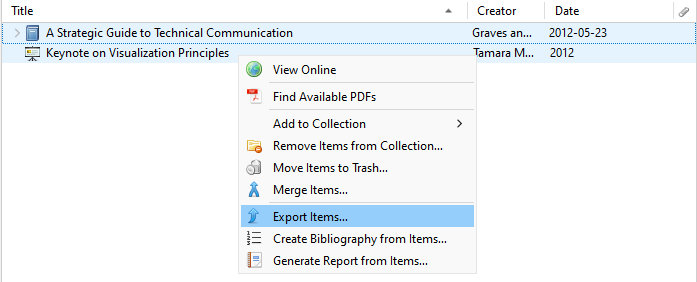
\includegraphics[width=\textwidth]{figures/Figure3-ZoteroBibliographyExport.png}
    \caption{The context menu of chosen sources in Zotero.}
    \label{fig:zoteroContext}
\end{figure}

After this, Zotero exports your chosen sources into a \verb|.bib|. The contents of that file you can copy into the \verb|references.bib| file in this environment. After that, referencing those sources in your text is already working. For each source, Zotero assigns a short label, which you can use to reference it. For example, the command \verb|\cite{tamara_munzner_keynote_2012}| has been used to create a reference to Tamara Munzner's lecture in this template.

The referenced scientific papers usually have Document Object Identifier (DOI) numbers. Specific DOI links\footnote{\url{https://dx.doi.org/}} (in the form doi.org/[number]) are generated from these. When referencing scientific papers, it is recommended to add the DOI links to the reference without the access date. When adding source links, ensure the links are correct and working. When You use the university proxy to access the papers, Your links directly on the browser’s address bar could be proxy links. Do not copy these into Your thesis. Ensure that Your reference links are clean and working, and, when possible, prefer the DOI links.

\subsection{Appendices}
The Appendices section in Your thesis follows the References section. In that part You can present larger tables or screenshots that do not fit in the main contents. Often, it is reasonable to present Your Glossary to define the jargon terms used in Your thesis. If You have created software during Your work, the Appendices section can also include the installation instructions and user manual. The section can be subsectioned and numbered in Your preferred way. For example, Appendix I: Glossary or Appendix B – User Manual, etc. There are many guides to creating a good user manual, but one example of writing technical texts is the textbook „A Strategic Guide to Technical Communication“ by Graves and Graves~\cite{graves_strategic_2012}.

One very important appendix is the description of the accompanying files. Together with the thesis document, You can also add an archived file. That archive file usually includes longer texts (for example, if Your user manual is very long, You need to include longer license texts for the user assets, the questionnaire used in Your study, etc.), larger files (for example, the measured raw data, their analysis files, audio and video recordings of the software or its testing, etc.), the created software, its source code, design concepts and other files created during Your work. Use one of the appendices to describe the contents of the accompanying files.

\subsection{License} \label{subchapter:license}
After the Appendix section, at the end of Your document, You must add a license to allow the  University of Tartu to store and distribute Your thesis. The text of that license is updated often and depends on whether Your work is classified or not. The newest texts are at the URL:  \url{https://adr.ut.ee/?page=pub_list_dynobj&desktop=57835&tid=70993&data_only=true&search=Otsi&field_100193_search_type=ANY&field_100193_text_search_value=ppimine}

The link above has the non-exclusive license as document number 30. In most cases, that license should apply to You. When Your work includes information that must not be published during some timeframe or even indefinitely, You need to write a corresponding application to the vice dean for academic affairs to use a limiting license. The application is in document number 32, and when the vice dean of academic affairs has approved Your application, You can use the corresponding limiting license from document number 31.

\subsection{Metadata}
Your thesis file includes metadata – data about the file itself. This template adds them automatically based on the fields you have written in the \verb|thesis.tex| file. You can see the metadata of a PDF file with the Acrobad Reader software, when you choose \emph{Document Properties} from the context menu of the opened document (see Figure~\ref{fig:metadata}). It is important that the metadata of your work correspond to reality.

\begin{figure}[ht]
    \centering
    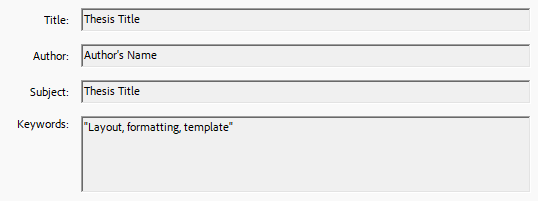
\includegraphics[width=0.8\textwidth]{figures/Figure4-Metadata.png}
    \caption{The metadata of the tempalte in Acrobat Reader.}
    \label{fig:metadata}
\end{figure}

It is recommended that You check through the rest of the metadata to ensure it is all good. For example, it has happened that the author of the file has not been the author of the thesis. This kind of contradiction creates suspicion about who has really authored the thesis document.

\section{Background}  \label{Background}



\subsection{Autonomous Driving Systems} \label{Background:AutonomousDrivingSystems}

% thesis: Autonomous Driving Systems have high safety requirements.

Autonomous Driving Systems (ADS), defined by the Society of Automotive Engineers (SAE) as the hardware and software that are collectively capable of performing the entire dynamic driving task (DDT) on a sustained basis, should have a high safety requirements.
This term is used to describe the three most advanced Levels 3 (Conditional), 4 (High), and 5 (Full) driving automation system \cite{sae:j3016:2021apr}. Additionally, ADS must be capable of operating under diverse operational conditions, defined as the operational design domain (ODD) \cite{sae:j3016:2021apr}. The ODD includes, but is not limited to, environmental, geographical, and time-of-day conditions.
While operating under these diverse conditions, ADS can experience DDT performance-relevant system failures that prevent it from reliably performing the DDT on a sustained basis.
In such cases, the ADS must issue a request to intervene, either for the user to perform the DDT or for the system to achieve a minimal risk condition.
At Level 3, a DDT fallback-ready user is expected to take over the DDT when a DDT performance-relevant system failure occurs or when the ADS is about to leave its operational design domain (ODD). This user must be receptive and able to resume DDT performance when alerted to do so.
For example, a Level 3 ADS experiences a DDT performance-relevant system failure in one of its radar sensors, which prevents it from reliably detecting objects in the vehicle's pathway. The ADS responds by issuing a request to intervene to the DDT fallback-ready user. The ADS continues to perform the DDT, while reducing vehicle speed, for several seconds to allow time for the DDT fallback-ready user to resume operation of the vehicle in an orderly manner. It is important to highlight that a key expectation for Level 3 ADS is the capability of continuing to perform the DDT for at least several seconds after issuing the fallback-ready user with a request to intervene.
For Levels 4 and 5 ADS, if a driving automation system can perform the entire DDT and DDT fallback either within a prescribed ODD (Level 4) or in all driver-manageable on-road operating situations (Level 5), then any users present in the vehicle while the ADS is engaged are passengers. For example, if a Level 4 ADS experiences a DDT performance-relevant system failure in one of its computing modules, it transitions to DDT fallback by engaging a redundant computing module(s) to achieve a minimal risk condition.
The high safety requirements defined by SAE imply significant robustness expectations for ADS. This means that an ADS should be capable of, first, performing the DDT for a few seconds following a performance-relevant system failure until DDT fallback, and second, in the case of Levels 4 and 5, it must be able to reach a minimal risk condition despite such a system failure \cite{sae:j3016:2021apr}.

% goal: explain relevance between sensors and video object detection task

ADS should be capable of perceiving data from various sources. The DDT is defined as all real-time operational and tactical functions required to operate a vehicle in on-road traffic. Object and Event Detection and Response (OEDR) refers to the subtasks of the DDT that include monitoring the driving environment (detecting, recognizing, and classifying objects and events, and preparing to respond as needed) and executing an appropriate response to such objects and events (i.e., actions required to complete the DDT and/or DDT fallback) \cite{sae:j3016:2021apr}. Performing the OEDR is necessary to complete the DDT and DDT fallback, and the capability of a Driving Automation System to handle OEDR allows it to be classified as Level 3 automation or higher. OEDR is also known as perception and a variety of computer vision tasks fall under this category, such as object detection, semantic segmentation, 3D object detection, and others.

OEDR tasks rely on exteroceptive sensors for perception hardware, which can be susceptible to system failures that can compromise overall system safety. ADS system architecture is predominantly realized with two approaches: modular or end-to-end \cite{yurtseverSurveyAutonomousDriving2020}. In both approaches, pipelines start with feeding raw sensor inputs to downstream system, either localization and object detection modules or an end-to-end model see the Figure \ref{fig:figure_background_ads_system_architecture}. Exteroceptive sensors, mainly used for commonly employed modalities for perceiving the environment, include cameras, LiDAR (light detection and ranging), radar, and ultrasonic sensors. These sensors vary in technologies and may exhibit various failures \cite{matosSurveySensorFailures2024}. The scope of this thesis will specifically investigate two critical failure modes: (1) non-deterministic sensor input availability, where the system receives inconsistent or temporally varying subsets of data from its sensors, and (2) the complete failure of a sensor component, where it provides no signal. Temporal Calibration, a mitigation strategy, establishes the synchronization rate of multiple sensor data streams \cite{matosSurveySensorFailures2024}. While Temporal Calibration aims to mitigate the first failure mode of non-deterministic sensor input, it cannot rule it out completely. This limitation stems from the asynchronous publish-subscribe communication model inherent in common ADS middleware frameworks like the Robot Operating System (ROS). In such systems, message delivery times for sensor data are not strictly guaranteed and can be influenced by variable factors including network latency, system processing load, and underlying operating system scheduling priorities. Consequently, even when employing ROS tools designed for time synchronization, these inherent timing uncertainties and potential for message delays or drops mean that perfect, deterministic, real-time alignment of all sensor data streams cannot always be achieved, leaving residual non-determinism in sensor input availability \cite{parkRealTimeCharacteristicsROS2020}. The complete sensor failure has no mitigation strategy except sensor redundancy \cite{matosSurveySensorFailures2024}.

\begin{figure}
    \centering
    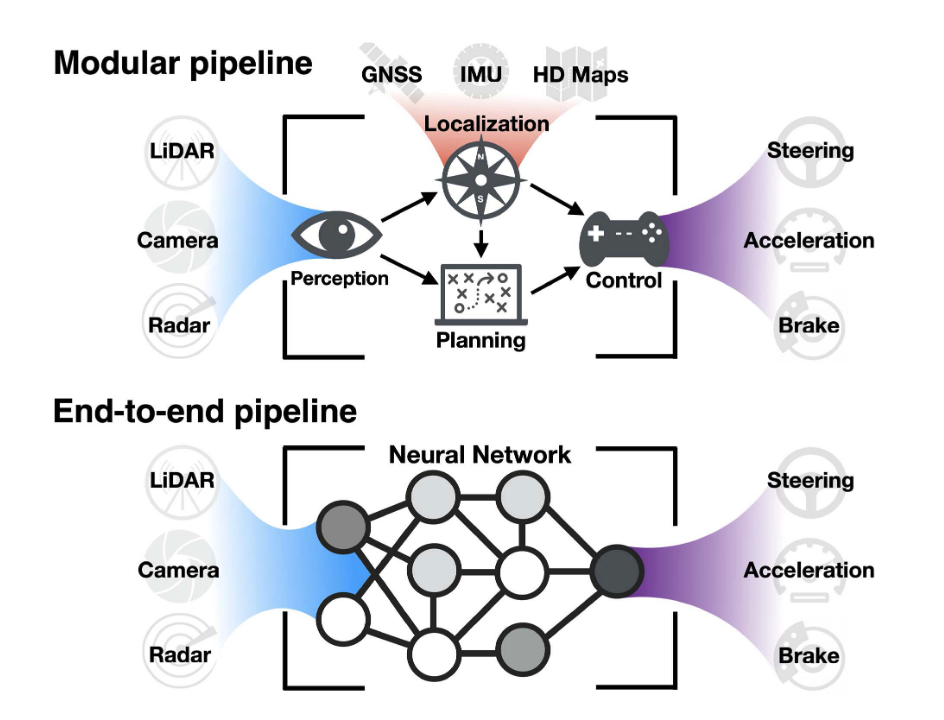
\includegraphics[width=\textwidth]{figures/figure_background_ads_system_architecture.png}
    \caption{Information flow diagrams of: (a) a generic modular system, and (b) an end-to-end driving system \cite{yurtseverSurveyAutonomousDriving2020}.}
    \label{fig:figure_background_ads_system_architecture}
\end{figure}

\subsection{Video Object Detection} \label{Background:VideoObjectDetection}

% Object detection definition. Deep learning pushed performance of single image object detection.

%TODO: add more exampleas of the progress in CV (from Object Detection from Video Tubelets with Convolutional Neural Networks)
Object detection is a foundational challenge in computer vision and has been a subject of research for several decades \cite{fischlerRepresentationMatchingPictorial1973}. The goal of the object detection task is to find objects of a given description in images and videos.
Advancements in deep learning techniques for feature representation learning \cite{hintonReducingDimensionalityData2006, lecunDeepLearning2015}, in conjunction with the significant development and application of deep Convolutional Neural Networks (CNN), have driven remarkable progress in various computer vision tasks, such as image classification \cite{krizhevskyImageNetClassificationDeep2012}, object detection \cite{girshickRichFeatureHierarchies2014a}.
Extending detection capabilities from static images to video sequences introduces the task of video object detection, which involves not only localizing objects within each frame but also leveraging temporal information across frames for improved accuracy and consistency.
The introduction of specific challenges, such as the video object detection track in the ImageNet Large Scale Visual Recognition Challenge (ILSVRC) \cite{russakovskyImageNetLargeScale2015}, provided benchmark datasets and standardized evaluation protocols, significantly accelerating research and development in the video object detection domain.

% State-of-the-Art
% Still-image detector
Due to the inherent similarity between detecting objects in single images and in video frames, the most straightforward approach to video object detection task is to apply a single-image object detector independently to each frame. 
This method, often referred to as frame-by-frame detection, treats each frame as independent image. %TODO: add citation where it's refered as f-to-f
However, such an approach ignores the rich temporal and contextual information available across consecutive video frames. Neglecting this temporal dimension often leads to suboptimal performance, characterized by issues like inconsistent bounding box predictions across frames, flickering detections, and reduced robustness to challenges specific to video, such as motion blur, occlusion, morphological diversity, and illumination variations within the video \cite{jiaoNewGenerationDeep2022}. 
Consequently, while applying static detectors frame-by-frame serves as a simple baseline, it is generally not considered an effective or optimal solution for the complexities of video object detection. %TODO: Add citation with examples

% For example, if an object is detected in neighboring frames but not in the current frame, we can recover the missing object in the current frame by applying temporal coherence.
% Another example is that mistakenly-labeled objects can be corrected by checking the semantic labels across the frames.

Video object detection algorithms can be broadly classified based on their architectural solution to the video object detection task. For this thesis, the classification proposed by the survey \cite{jiaoNewGenerationDeep2022} is adopted. This survey categorizes these algorithms into four main types: those based on image detection (postprocessing methods), those utilizing motion information (introducing additional models), those employing feature filtering, and other effective network structures.

\begin{figure}
    \centering
    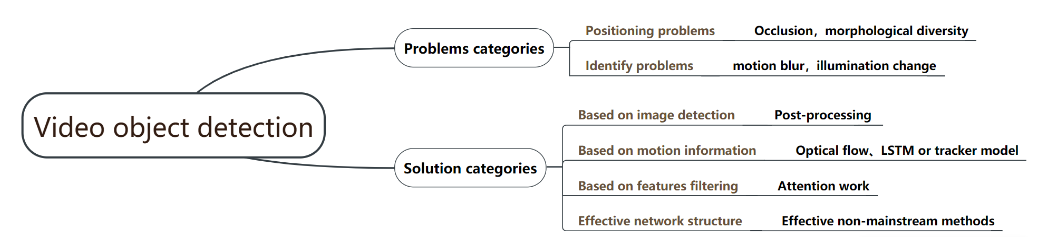
\includegraphics[width=\textwidth]{figures/figure_background_vod_classification.png}
    \caption{Classification of video object detection problems and solutions \cite{jiaoNewGenerationDeep2022}.}
    \label{fig:figure_background_vod_classification}
\end{figure}

% Postprocessing (not e2e)
% T-CNN: ImageNet VID 2015 73 - 77 mAP
One strategy involves applying a postprocessing step to the outputs of a still-image detector to enhance temporal consistency \cite{hanSeqNMSVideoObject2016, kangTCNNTubeletsConvolutional2018, kangObjectDetectionVideo2016}. This often utilizes detections from adjacent frames to refine the results for the current frame. Common postprocessing techniques include Sequence Non-Maximum Suppression (Seq-NMS), which links high-scoring detection boxes across frames into sequences \cite{hanSeqNMSVideoObject2016}, or leveraging optical flow to propagate detection scores \cite{kangTCNNTubeletsConvolutional2018, kangObjectDetectionVideo2016}. While these methods can improve upon static image detectors, exploiting temporal information solely during postprocessing is considered suboptimal, as crucial temporal and motion cues are disregarded during the primary detector training phase. Therefore, such algorithms have difficulty overcoming consecutive failures of the static image detector when the object of interest experiences long-term occlusions or significant appearance changes.

% motion information

To address the limitation of postprocessing, another category of methods utilizing motion information by introducing additional models to integrate motion and temporal information directly into the model training, often creating end-to-end solutions. This category is subdivided into models based on optical flow, contextual information, and trajectory information. For the purpose of this thesis, a subcategory of contextual information is reviewed, which utilizes Recurrent Neural Networks (RNN) and their variants. The power of RNNs in long-range temporal representation has become a valuable tool for the video object detection task \cite{Lu_2017_ICCV, xiaoVideoObjectDetection2018, liuMobileVideoObject2018}, enabling the design of end-to-end networks. One of the challenges posed by such methods is how to associate objects within the RNN structure across multiple frames.

One notable early attempt to tackle this association problem is the Association LSTM framework \cite{Lu_2017_ICCV}. The framework consists of an SSD image detector \cite{liuSSDSingleShot2016} and a variant of the RNN model, the Long Short-Term Memory (LSTM) network \cite{6795963}. SSD detects frame-wise, image-based object detection results (bounding box, score, and object feature) which are stacked and fed into the LSTM. The association LSTM not only regresses and classifies directly on object locations and categories but also associates features to represent each output object. By minimizing the matching error between these features, the network learns how to associate objects in two consecutive frames. Additionally, the method works in an online manner, which is important for real-world applications. The authors acknowledge that a weakness of these frameworks is that the LSTM module is a post-hoc addition, since performance is limited by the quality of the initial SSD detections. Missed or poorly localized detections by the SSD are difficult for the LSTM to recover. Furthermore, the SSD parameters are not updated during training.

% T-CNN with LSTM
% TUBELETS: ImageNet VID 2015 ~75ish mAP

% % STMN: ImageNet VID 2015 80.5 mAP
Building upon the idea of modeling temporal dependencies but aiming for deeper integration and leveraging spatial information more effectively, the Spatial-Temporal Memory Network (STMN) was proposed \cite{xiaoVideoObjectDetection2018}. Unlike the Association LSTM which operates on vector-form features within a standard LSTM, STMN introduces a Spatial-Temporal Memory Module (STMM). This module utilizes a modified bidirectional convolutional Gated Recurrent Unit (ConvGRU) \cite{ballasDelvingDeeperConvolutional2016}, allowing it to process and retain information in a spatially structured manner directly from convolutional feature maps generated by the detector backbone. By preserving spatial locality within the recurrent computation, STMM can better capture appearance changes and motion patterns. Experimental results indicated that the effectiveness of such convolutional memory modules increases with the length of the input sequence, as more relevant long-range context can be accumulated, leading to improved detection accuracy, particularly for challenging scenarios involving occlusion or significant appearance variations \cite{xiaoVideoObjectDetection2018}.

The principle of using convolutional recurrent units to efficiently propagate spatio-temporal information proved beneficial not only for accuracy but also for enabling real-time video object detection on resource-constrained platforms. In this work \cite{liuMobileVideoObject2018}, an architecture is introduced that augments a single-image object detector (SSD with a pruned MobileNet base) by interweaving efficient convolutional LSTM (ConvLSTM) \cite{} layers, specifically "Bottleneck-LSTM" layers, to refine and propagate feature maps across frames. Despite its more complex architecture, an array of modifications is proposed that allow this model to be faster and more lightweight than mobile-focused single-frame models.

% Feature filtering

Another category of video object detection methods employs feature filtering techniques to enhance performance by selectively focusing on relevant spatiotemporal information while suppressing redundant or irrelevant data. This approach draws inspiration from the human visual system, which can rapidly identify salient regions within a scene, thereby optimizing cognitive resources for efficient analysis \cite{}. Similarly, feature filtering mechanisms in neural networks aim to prioritize critical features and reduce unnecessary computations, leading to improvements in both accuracy and efficiency \cite{jiaoNewGenerationDeep2022}. These methods can be broadly subdivided based on the specific filtering mechanism employed, notably attention mechanisms \cite{bahdanauNeuralMachineTranslation2016a, vaswaniAttentionAllYou2023} and deformable convolutions \cite{}.

Attention mechanisms allow networks to dynamically weigh the importance of different features or spatial locations across video frames. This selective focus enables the propagation of crucial information, particularly for objects undergoing significant appearance changes or movements, potentially offering advantages over methods relying solely on adjacent frame correlations or optical flow, which can struggle with large displacements and add significant model complexity \cite{jiaoNewGenerationDeep2022, guoProgressiveSparseLocal2019}.

One prominent example is the Progressive Sparse Local Attention (PSLA) framework \cite{guoProgressiveSparseLocal2019}. Addressing limitations associated with optical flow, such as increased model size and difficulty handling large displacements or high-level features, PSLA provides an alternative mechanism for establishing feature correspondence and propagating information between frames \cite{guoProgressiveSparseLocal2019}. Instead of calculating pixel-level flow, PSLA operates directly on feature maps. While similar to STMN \cite{xiaoVideoObjectDetection2018} which also uses local correlation for alignment, PSLA differs by utilizing a sparse neighborhood and softmax normalization for better spatial correspondence, aiming to improve both speed and accuracy \cite{guoProgressiveSparseLocal2019}. It uses a special attention approach called progressive sparse stride, which pays more attention to nearby features (for small movements) and less attention to features farther away (for larger movements). By calculating weighted correspondences based on feature similarity within this sparse local neighborhood, PSLA aligns and aggregates features across time, enabling temporal feature updating and enhancement without relying on an explicit optical flow model. This approach aims to achieve a better balance between accuracy, speed, and model size compared to traditional flow-based methods \cite{guoProgressiveSparseLocal2019}. Nevertheless, managing the complexity of attention calculations remains a factor.

More recently, Transformer architectures \cite{vaswaniAttentionAllYou2017} have demonstrated significant potential in computer vision tasks, including object detection \cite{carionEndToEndObjectDetection2020, zhuDeformableDETRDeformable2021}. Models like DETR (DEtection TRansformer) \cite{carionEndToEndObjectDetection2020, zhuDeformableDETRDeformable2021} and its derivatives aim to simplify the traditional detection pipeline by reformulating object detection as a set prediction problem, eliminating the need for hand-designed components like NMS or anchor generation found in many CNN-based detectors. While newer to video object detection compared to RNNs, Transformers offer a different paradigm for modeling long-range dependencies and object relationships within sequences \cite{wangEndtoEndVideoObject2021, shvetsTrackingObjectsAs2021}.

\subsection{General Purpose Perceiver Model} \label{Background:Perceiver}

Most architectures used by AI systems today are specialized. For instance, models presented in \ref{Background:VideoObjectDetection} built for the video object detection task might excel at processing 2D video frames, but they are hardly ideal for other data types, such as the LiDAR point clouds or radar output used in ADS. Handling multiple data modalities, like the sounds and images that make up videos, presents even greater complexity and usually involves complex, hand-tuned systems built from many different parts, even for simple tasks. Real-world problems, such as building an ADS, possess these complexities, so there is a desperate need to build a simple yet effective, more general, and versatile architecture that can handle all types of data.

Perceiver \cite{jaeglePerceiverGeneralPerception2021} was introduced as a general-purpose architecture that is capable of processing different data types such as images, point clouds, audio, video, and, what is important, combinations of those to fuse together. The Perceiver builds upon the Transformer \cite{vaswaniAttentionAllYou2023}, an architecture that uses an operation called "Attention" to map inputs into outputs \cite{bahdanauNeuralMachineTranslation2016a}. While attention is simple and widely applicable, the way Transformers utilize attention can become memory expensive as the number of inputs grows. Consequently, Transformers perform well with inputs containing at most a few thousand elements, but common data forms like images and videos can easily comprise millions of elements. This fact poses a challenge to the generalist architecture: scaling the Transformer's attention operation to very large inputs without introducing domain-specific assumptions. The Perceiver addresses this by using attention to first encode the inputs into a small latent array. This latent array can then be processed further at a cost independent of the input's size, allowing the Perceiver's memory and computational needs to scale gracefully as the input size grows, even for particularly deep models. This "graceful growth" enables the Perceiver to achieve an unprecedented level of generality - it is competitive with domain-specific models on benchmarks based on images, 3D point clouds, and combined audio and images \cite{jaeglePerceiverGeneralPerception2021}.

\begin{figure}
    \centering
    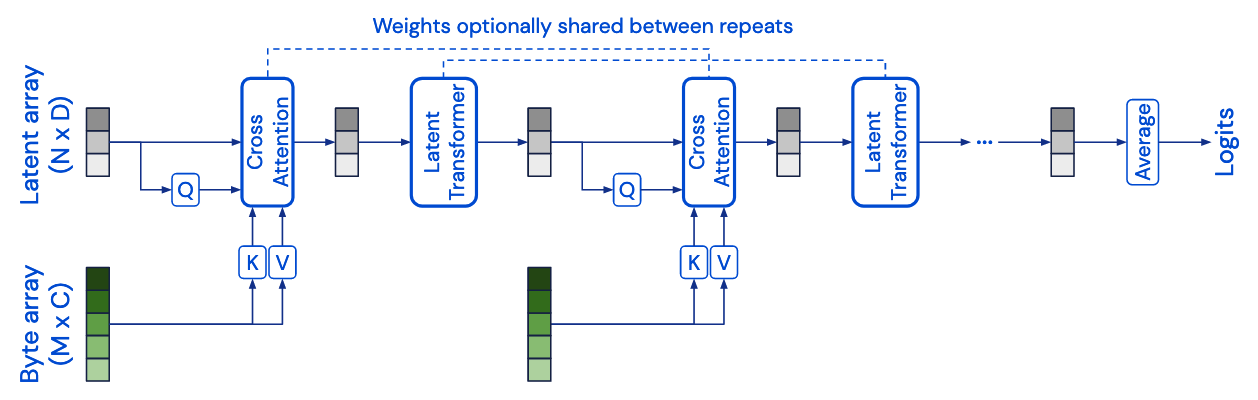
\includegraphics[width=\textwidth]{figures/figure_background_perceiver_architecture.png}
    \caption{The Perceiver is an architecture based on attentional principles that scales to high-dimensional inputs such as images, videos, audio, point-clouds, and multimodal combinations without making domain-specific assumptions. The Perceiver uses a cross-attention module to project an high-dimensional input byte array to a fixed-dimensional latent bottleneck (the number of input indices M is much larger than the number of latent indices $N$) before processing it using a deep stack of Transformer-style self-attention blocks in the latent space. The Perceiver iteratively attends to the input byte array by alternating cross-attention and latent self-attention blocks \cite{jaeglePerceiverGeneralPerception2021}.}
    \label{fig:figure_background_perceiver_architecture}
\end{figure}

The Perceiver architecture consists of two primary components: (i) a cross-attention module that maps an input byte array (e.g. a pixel array) and a latent array to an updated latent array, and (ii) a Transformer tower that maps this latent array to another latent array \cite{jaeglePerceiverGeneralPerception2021}. The Perceiver architecture is illustrated in Figure \ref{fig:figure_background_perceiver_architecture}. The model can be conceptualized as a recurrent neural network (RNN) unrolled in depth with the same input, rather than unrolled in time. A central challenge addressed by this architecture is the scaling of attention mechanisms to accommodate very large and diverse inputs. The Perceiver mitigates the quadratic complexity bottleneck inherent in standard Transformers by employing its cross-attention module. This module introduces an asymmetry into the attention operation when applied directly to the inputs.

Specifically, for a query $Q \in \mathbb{R}^{M \times D}$, key $K \in \mathbb{R}^{M \times C}$, and value $V \in \mathbb{R}^{M \times C}$ (where $C$ and $D$ represent channel dimensions), the computational complexity of the standard $QKV$ attention operation---formulated as $\text{softmax}(QK^T)V$---is $\mathcal{O}(M^2)$. This is due to matrix multiplications involving the large input index dimension $M$. The authors of Perceiver introduced an asymmetry: while $K$ and $V$ are projections of the input byte array (with $M$ elements), $Q$ is a projection of a learned latent array characterized by a much smaller index dimension $N \ll M$. The dimension $N$ of this latent array is a hyperparameter. Consequently, the resulting cross-attention operation exhibits a complexity of $\mathcal{O}(MN)$. It is important to note that within the Perceiver's cross-attention, linear projection layers are applied to generate $Q$, $K$, and $V$ such that they share a common channel dimension before the attention calculation.

This design enables Perceiver-based architectures to leverage significantly deeper Transformers compared to efficient Transformer variants that use linear complexity layers, without depending on domain-specific assumptions. Using $L$ to represent the number of layers in the Transformer tower, the complexity of a standard Transformer operating directly on $M$ input elements (bytes) can be represented as $\mathcal{O}(LM^2)$, whereas the complexity of Perceiver's latent Transformer (processing the $N$-dimensional latent array) is $\mathcal{O}(LN^2)$. Given that $N \ll M$, this substantially reduces the computational cost per layer. The overall architecture's complexity thus becomes $\mathcal{O}(MN + LN^2)$ for a latent Transformer with $L$ layers. This decoupling of the input size from the network depth is crucial, as it permits the addition of Transformer layers at a cost that is independent of the input size.

However, because the original Perceiver produced only one output per input, it was not as versatile as researchers required. Our proposed architecture aims to address this limitation by modifying the Perceiver architecture to make it akin to a recurrent unit processing input over time.



\section{Methods}  \label{Methods}

In this section We propose a novel RNN architecture called the Recurrent Perceiver to model an object's changing appearance and motion over time for video object detection.
This section outlines the procedure used for training the models presented in this thesis.

\subsection{Model} \label{Methods:Model}

We introduce a new Recurrent Perceiver (RPerceiver), a Recurrent Neural Network (RNN) capable of processing high-dimensional inputs. This architecture is inspired by the Perceiver \cite{jaeglePerceiverGeneralPerception2021} due to its ability to handle high-dimensional data.
We have re-engineered the Perceiver architecture by adding a temporal dimension, effectively unrolling it over time. This addresses the original Perceiver's limitation of producing only a single output per input, which makes it unsuitable for tasks with a temporal component, such as video object detection. If previously, the Perceiver was only unrolled in depth, now we have closed the loop and unrolled it in time by propagating the latent array between time steps. For the initial time step, we still use a learnable latent array, similar to the original Perceiver \cite{jaeglePerceiverGeneralPerception2021}.
The architecture of the RPerceiver is illustrated in Figure \ref{fig:figure_methods_recurrent_perceiver}.

\begin{figure}
    \centering
    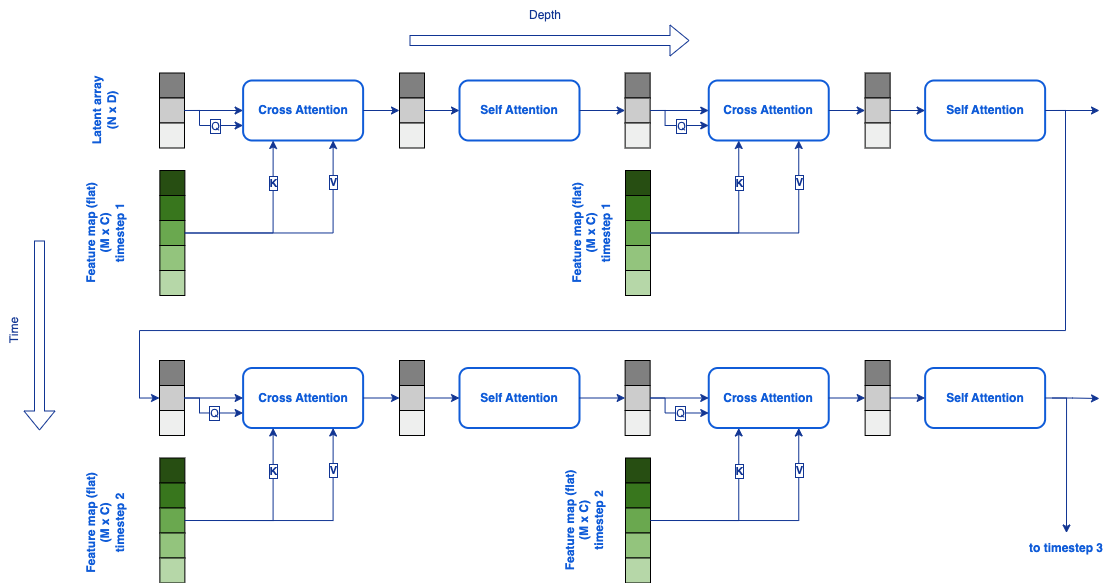
\includegraphics[width=\textwidth]{figures/figure_methods_recurrent_perceiver.png}
    \caption{The Recurrent Perceiver (RPerceiver) architecture. The model processes inputs along the time dimension by propagating the latent array between time steps. In the depth dimension (within a single time step), this example shows two processing blocks, similar to the original Perceiver, applied to the input and latent arrays.}
    \label{fig:figure_methods_recurrent_perceiver}
\end{figure}

% TODO: Read about calibration problem.

We propose a variation of the RPerceiver architecture capable of processing multi-modal inputs, which we call the Recurrent Perceiver Multi-Modal (RPerceiverMM). The original Perceiver paper \cite{jaeglePerceiverGeneralPerception2021} handled multi-modality by concatenating a learned, modality-specific encoding to each input element. Modern Autonomous Driving Systems (ADS) process information from multiple sensors, often including multiple cameras placed in different locations, which presents a calibration challenge. Therefore, our work adopts a different approach to multi-modality. We introduce a camera-specific cross-attention module to the RPerceiverMM. Within the scope of this thesis, we focus on a multi-view camera setup. The architecture of the RPerceiverMM is illustrated in Figure~\ref{fig:figure_methods_model_ar_perceiver_views}.

% TODO edit fiture and name

\begin{figure}
    \centering
    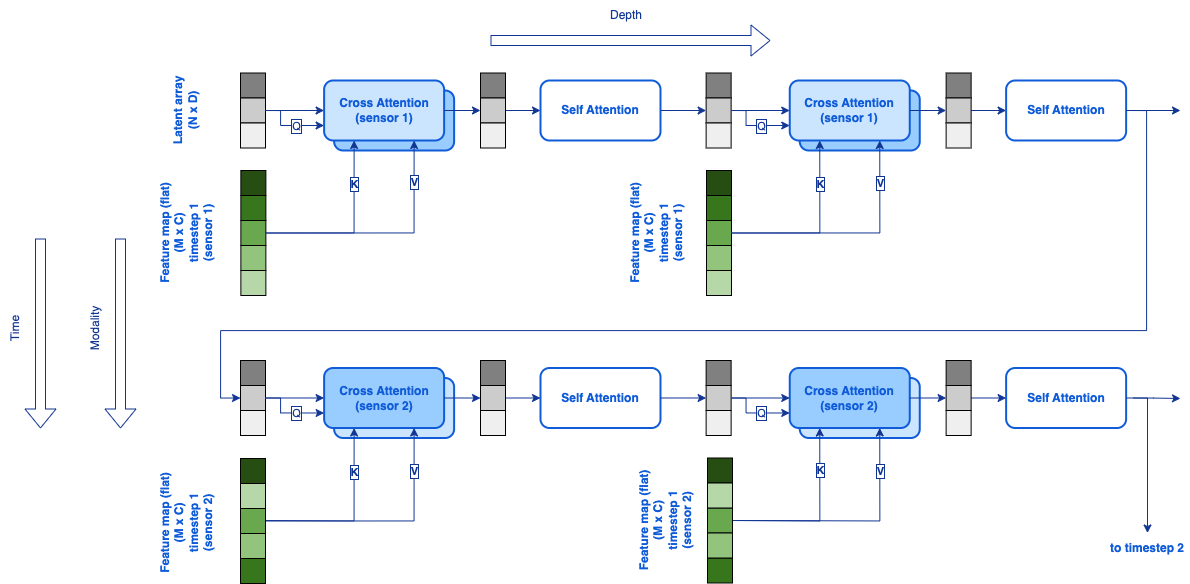
\includegraphics[width=\textwidth]{figures/figure_methods_recurrent_perceiver_mm.png}
    \caption{The Recurrent Perceiver Multi-Modal (RPerceiverMM) architecture designed for multi-view camera inputs. It employs camera-specific cross-attention modules to process information from different sensors (views). In this example, separate cross-attention blocks are used for each camera input, integrating modality-specific information.}
    \label{fig:figure_methods_recurrent_perceiver_mm}
\end{figure}

In addition to the RPerceiver module, we used a CNN backbone to learn a 2D representation of the input frames. We designed this backbone consisting of four blocks with convolutional layers and ReLU activation. Each block progressively downscales spatial dimensions by a factor of 2 while increasing channel dimensionality, resulting in a final feature map with 128 channels and $\frac{1}{16}$ of the original spatial resolution.
The output features from the RPerceiver module are passed to the detection heads, which are responsible for predicting object labels and positions. We employed detection heads the same as those in the DETR model \cite{carionEndtoEndObjectDetection2020}. These heads include a linear layer to predict the class label using a softmax function and a 3-layer Multi-Layer Perceptron (MLP) with ReLU activation function to predict object coordinates. We considered two variants for object coordinates: (i) bounding boxes, where the MLP predicts the normalized center coordinates, height, and width relative to the input image, and (ii) center points. The corresponding output dimensions are $N \times 4$ and $N \times 2$, respectively, where $N$ is a fixed number of detection slots (queries). Since $N$ is typically much larger than the actual number of objects, a special class label $\emptyset$ is used to indicate that no object is detected within a slot, playing a role similar to a background class.
For bounding boxes, we used a sigmoid activation function to predict the normalized coordinates of the bounding box center, as well as its width and height. For center points, we used a tanh activation function. This choice was made because we placed the origin of the coordinate system at the center to mimic a bird's-eye view, similar to an ADS positioned centrally with surrounding views.
The complete architecture of the model is shown in Figure~\ref{fig:figure_methods_model_r_perceiver_complte}.

% TODO edit fiture and name

\begin{figure}
    \centering
    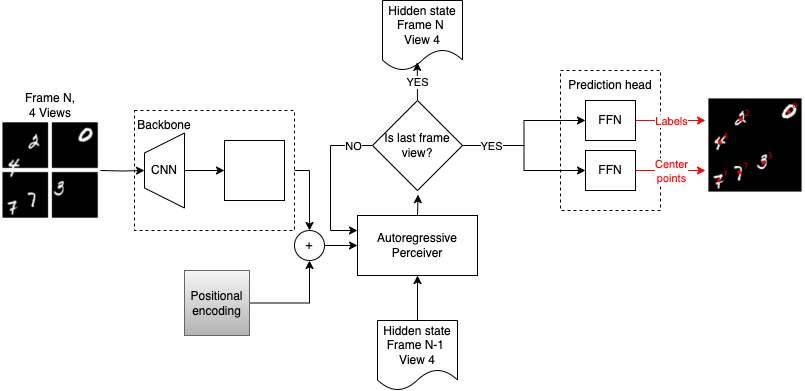
\includegraphics[width=\textwidth]{figures/figure_methods_model_ar_perceiver_views.png}
    \caption{Full architecture of our model. The backbone output is supplemented with a learned view-specific positional encoding before passing it to the autoregressive Perceiver model. The autoregressive Perceiver takes a hidden state from the previous frame's last view and iterates through the current frame's views. After the last view, we pass the output embedding of the Perceiver to the feed-forward network (FFN) that predicts class labels and center points on the global frame raster.}
    \label{fig:figure_methods_model_r_perceiver_complte}
\end{figure}


\subsection{Dataset} \label{Methods:Dataset}

For our experiment, we generated our own dataset, which we call "detection-moving-mnist-easy". We took inspiration from the MovingMNIST dataset \cite{srivastava2016unsupervisedlearningvideorepresentations}, which is used for TODO use cases. In our case, we are interested in video object detection and a simplified variation of keypoints, where we predict a center point of the object it is similar to keypoints task because the center of object is not the same as center of the bounding box. We hosted the dataset on Hugging Face \footnote{\url{https://huggingface.co/datasets/Max-Ploter/detection-moving-mnist-easy}}.

 For the first frame, we pick a number of digits from 1 to 10 with uniform probability (see Figure~\ref{fig:figure_method_dataset_train_digit_classes}). Depending on the number of digits per first frame, we draw, without replacement, from the well-known MNIST dataset \cite{} (from the train and test splits corresponding to the dataset split). Each digit is placed on the first frame of the canvas image of size 128x128. There's a greedy algorithm that places digits on the first frame randomly and tries to avoid overlaps, so it's easier for the model to detect all objects in the beginning. To each digit, we assign an affine translation from -5 to 5 randomly with uniform probability. Then, we apply corresponding affine transformations to move the digits through 20 frames on the canvas image of size 128x128. As a result, we receive a tensor of size 20x1x128x128, which represents a video (see Figure~\ref{fig:figure_methods_dataset_detection_mmnist_sequence}).

\begin{figure}
    \centering
    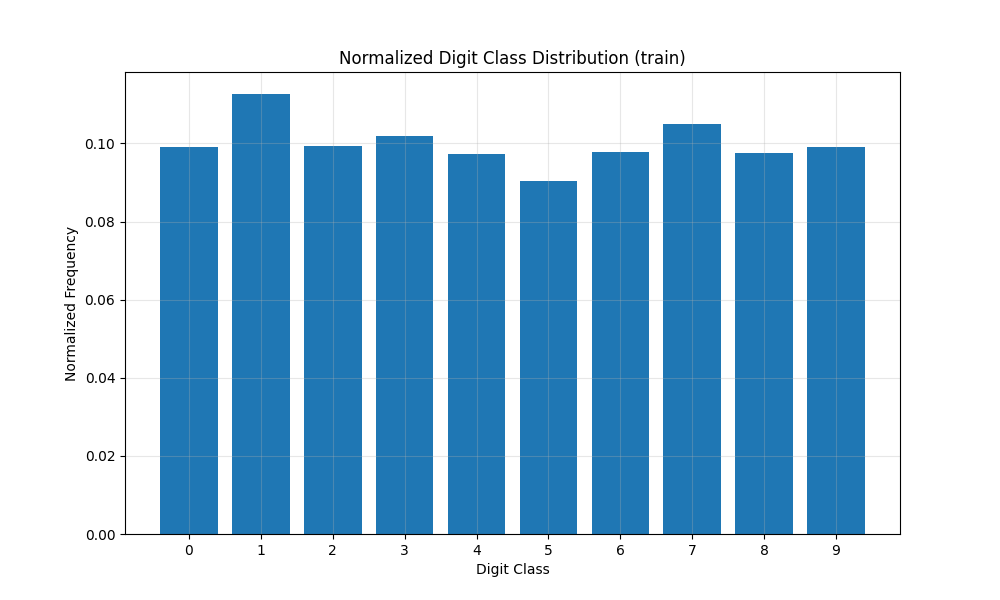
\includegraphics[width=\textwidth]{figures/figure_method_dataset_train_digit_classes.png}
    \caption{Distribution of classes in the "detection-moving-mnist-easy" dataset.}
    \label{fig:figure_method_dataset_train_digit_classes}
\end{figure}


\begin{figure}
    \centering
    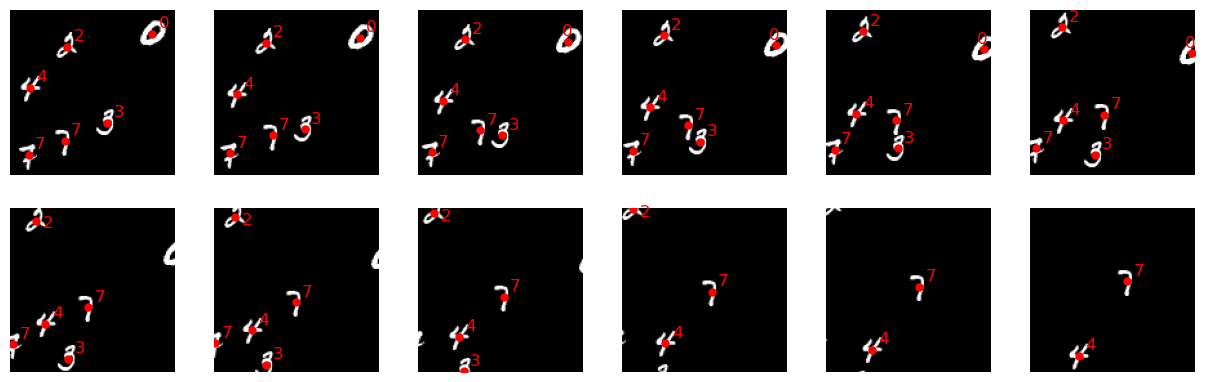
\includegraphics[width=\textwidth]{figures/figure_methods_dataset_detection_mmnist_sequence.png}
    \caption{Example of 12 frames from the sequence. Ground truth, shown in red, indicates the ground truth digit center point and a class label.}
    \label{fig:figure_methods_dataset_detection_mmnist_sequence}
\end{figure}


In order for dataset to be more challanging we do not restrict digit overlap in subsequent frames. It is even possible to have some degree of overlap in the first frame if the greedy algorithm is unable to randomly place digits in such a way on the first frame. We do not bounce digits against image boundaries, so each digit can leave the frame. You can see in the figure that later frames have fewer digits (see Figure~\ref{fig:figure_method_dataset_train_digits_per_frame}).

% TODO DOUBLE CHECK number this plot
\begin{figure}
    \centering
    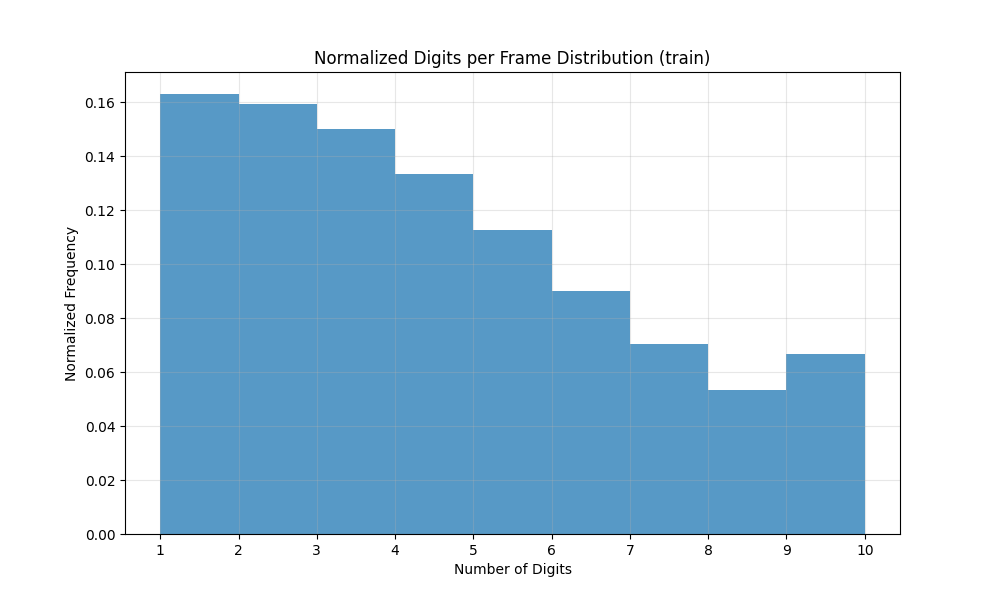
\includegraphics[width=\textwidth]{figures/figure_method_dataset_train_digits_per_frame.png}
    \caption{Distribution of classes in the "detection-moving-mnist-easy" dataset.}
    \label{fig:figure_method_dataset_train_digits_per_frame}
\end{figure}

We generated the dataset with 60K and 10K train and test splits, respectively. Annotations, automatically generated during sequence creation, include digit classes and digit center point coordinates (keypoint), bounding box coordinates and digit's identity ID.

\subsection{Metrics} \label{Methods:Metrics}

% TODO: mention mAP 75

We used mean Average Precision (mAP) as the primary metric to evaluate the model's performance. A widely used metric in object detection, mAP measures the average precision across various Intersection over Union (IoU) thresholds, adapted from information retrieval evaluation methods and popularized in challenges like PASCAL VOC \cite{everinghamPascalVisualObject2010}. Specifically, we report the mAP at an IoU threshold of 0.5, a common choice established in early object detection benchmarks such as PASCAL VOC \cite{everinghamPascalVisualObject2010}, and the mAP at 0.5-0.95, which represents the mean of the average precision calculated at IoU thresholds ranging from 0.5 to 0.95 with a step of 0.05, as introduced by the COCO challenge \cite{linMicrosoftCOCOCommon2015a}.

We used the Average Displacement Error (ADE) and Final Displacement Error (FDE) metrics to evaluate the model's performance. The ADE measures the average distance between the predicted and ground truth center points over the sequence of frames \ref{eq:ade}.

\begin{equation}
    \text{ADE} = \frac{1}{N \cdot T} \sum_{i=1}^{N} \sum_{t=1}^{T} || \hat{y}_{i,t} - y_{i,t} ||_2
    \label{eq:ade}
\end{equation}

The FDE measures the distance between the predicted and ground truth center points at the last frame of the sequence \ref{eq:fde}.

\begin{equation}
    \text{FDE} = \frac{1}{N} \sum_{i=1}^{N} || \hat{y}_{i,T} - y_{i,T} ||_2
    \label{eq:fde}
\end{equation}

\subsection{Loss Function} \label{Methods:LossFunction}

We adopted the loss calculation approach from DETR \cite{carionEndtoEndObjectDetection2020} and \cite{stewartEndtoendPeopleDetection2015}. The model (\ref{Methods:Model}) predicts a fixed-size set of $N$ potential objects per timestep. The parameter $N$ is a dimension of the latent array and is chosen to be greater than the cardinality of the largest set of ground-truth objects per frame. The model uses an attention mechanism that allows it to attend to all other elements in the attention map. Therefore, there is no predefined structure, like a grid in one-stage image detectors \cite{}, associating predictions with ground-truth objects. This presents the core challenge of how to score the fixed-size prediction set against the variable-size ground-truth set of objects. The loss function calculation consists of two steps: first, finding an optimal bipartite matching between the elements of the predicted and ground-truth sets, and second, calculating a loss.

Let us denote the set of predictions for a given timestep as $ \hat{Y} = \{\hat{y}_j\}_{j=1}^N $ and the corresponding set of ground-truth objects for that frame as $ Y = \{y_i\}_{i=1}^M $. At each recurrence (i.e., for each frame/timestep processed), the RPerceiver outputs the entire set of $N$ predictions $\hat{Y}$. Each prediction $\hat{y}_j \in \hat{Y}$ consists of a predicted object representation $\hat{o}_j$ and a predicted class label $\hat{c}_j$ (including the possibility of the no-object class $\emptyset$). The nature of $\hat{o}_j$ depends on the specific task:
\begin{itemize}
    \item For the \textbf{bounding box prediction task}, $\hat{o}_j$ is the predicted box $\hat{b}_j = (\hat{b}_x, \hat{b}_y, \hat{b}_w, \hat{b}_h) \in \mathbb{R}^4$, representing center coordinates, height, and width relative to the frame size.
    \item For the \textbf{center point prediction task}, $\hat{o}_j$ is the predicted center point coordinates $\hat{p}_j = (\hat{p}_x, \hat{p}_y) \in \mathbb{R}^2$ relative to the frame size.
\end{itemize}
Similarly, each ground-truth object $y_i \in Y$ consists of the ground-truth object representation $o_i$ (either a box $b_i$ or a point $p_i$) and the ground-truth class label $c_i$.
We define a matching algorithm via an injective function $f: Y \rightarrow \hat{Y}$, where $f(y_i)$ is the candidate hypothesis $\hat{y}_j \in \hat{Y}$ assigned to the ground-truth object $y_i$. Given $f$, we define a loss function on pairs of sets $Y$ and $\hat{Y}$ as \cite{}:
\begin{equation} \label{eq:set_loss}
L(Y, \hat{Y}, f ) = \sum_{i: f(y_i) \text{ is defined}} l_{pos}(y_i, f(y_i)) +  \sum_{j=1}^{N} l_c (\hat{y}_j, y_j^{\text{match}})
\end{equation}
where $l_c$ is the class prediction loss, for which we utilize the Focal Loss \cite{}, and $l_{pos}$ is an object localization loss. The formulation of $l_{pos}$ depends on the specific task (bounding box or center point). Details on each loss term are provided below.

\textbf{Focal Loss.} The Focal Loss is used to address the class imbalance between the foreground objects and the numerous potential background predictions. The class loss component $l_c$ for each prediction $\hat{y}_j$ is calculated using the sigmoid Focal Loss, summed over all foreground classes $k \in \{1, ..., C\}$, where $C$ is the number of object categories (excluding the $\emptyset$ class). The Focal Loss for a single class $k$ and prediction $j$ is defined as:
\begin{equation} \label{eq:focal_loss}
    \text{FL}(p_{jk}) = - \alpha_t (1 - p_{jk})^\gamma \log(p_{jk})
\end{equation}
where $p_{jk} = \sigma(x_{jk})$ is the predicted sigmoid probability for class $k$ from the raw logits $x_{jk}$, and $\alpha_t$ and $p_t$ are defined based on the ground-truth label $y_{jk}$ (which is 1 if the matched ground-truth class is $k$, and 0 otherwise):
\begin{equation*}
    p_t =
    \begin{cases}
        p_{jk} & \text{if } y_{jk} = 1 \\
        1 - p_{jk} & \text{if } y_{jk} = 0
    \end{cases}
\end{equation*}
The term $\gamma \ge 0$ is the focusing parameter, which reduces the relative loss for well-classified examples, thereby putting more focus on hard, misclassified examples. The term $\alpha_t$ is a weighting factor to address class imbalance, typically $\alpha$ for the positive class ($y_{jk}=1$) and $1-\alpha$ for the negative class ($y_{jk}=0$). The total class loss for prediction $j$ is $l_c(\hat{y}_j, y_j^{\text{match}}) = \sum_{k=1}^{C} \text{FL}(p_{jk})$. For unmatched predictions ($\hat{y}_j$ matched to $\emptyset$), $y_{jk}=0$ for all foreground classes $k$.

\textbf{Bounding Box Loss} is a linear combination of the L1 loss and the Generalized IoU (GIoU) loss \cite{}:
\begin{equation}
    \mathcal{L}_{box}(b_i, \hat{b}_j) = \lambda_{L1} \mathcal{L}_{L1}(b_i, \hat{b}_j) + \lambda_{giou} \mathcal{L}_{giou}(b_i, \hat{b}_j)
    \label{eq:box_loss_revised}
\end{equation}
where $y_i = (c_i, b_i)$ and $\hat{y}_j = (\hat{c}_j, \hat{b}_j)$, and:
\begin{itemize}
    \item $ \mathcal{L}_{L1}(b_i, \hat{b}_j) = \|b_i - \hat{b}_j\|_1 $ is the L1 norm, weighted by $ \lambda_{L1} $ (e.g., \texttt{weight\_dict['loss\_bbox'] * bbox\_loss\_coef}).
    \item $ \mathcal{L}_{giou}(b_i, \hat{b}_j) = 1 - \text{GIoU}(\text{box\_ops.box\_cxcywh\_to\_xyxy}(b_i), \text{box\_ops.box\_cxcywh\_to\_xyxy}(\hat{b}_j)) $, weighted by $ \lambda_{giou} $ (e.g., \texttt{weight\_dict['loss\_giou'] * giou\_loss\_coef}). GIoU is defined in \cite{Rezatofighi2019GeneralizedIO}. % Added GIoU citation
\end{itemize}
Both the $ \mathcal{L}_{L1} $ and $ \mathcal{L}_{giou} $ components are normalized by the total number of actual ground-truth boxes ($M$) across the batch (denoted as \texttt{num\_boxes}). Thus, for matched pairs in the bounding box task, $l_{pos}(y_i, \hat{y}_j) = \mathcal{L}_{box}(b_i, \hat{b}_j)$.

\textbf{Center Point Loss.} For the center point prediction task, the localization loss $l_{pos}(y_i, \hat{y}_j)$ applies \textit{only} to matched pairs $(i, j)$ where $f(y_i) = \hat{y}_j$. we use the L1 distance between the ground-truth center point $p_i$ and the predicted center point $\hat{p}_j$:
\begin{equation} \label{eq:point_loss}
    \mathcal{L}_{point}(p_i, \hat{p}_j) = \|p_i - \hat{p}_j\|_1
\end{equation}
where $y_i = (c_i, p_i)$ and $\hat{y}_j = (\hat{c}_j, \hat{p}_j)$. The total localization loss term in Equation \ref{eq:set_loss} for this task involves summing $\mathcal{L}_{point}$ over all matched pairs and normalizing by the total number of ground-truth objects ($M$) in the batch (denoted as \texttt{num\_objects}). Thus, for matched pairs in the center point task, $l_{pos}(y_i, \hat{y}_j) = \mathcal{L}_{point}(p_i, \hat{p}_j)$.

\textbf{Matching Function ($ f $):} This optimal assignment is computed efficiently using the Hungarian algorithm \cite{Kuhn1955TheHM, Carion2020EndToEndOD, Stewart2015EndtoendPD}. The pairwise matching cost $\mathcal{L}_{match}(y_i, \hat{y}_j)$ used within the Hungarian algorithm depends on the task. For the \textbf{bounding box task}, it is defined as \cite{Carion2020EndToEndOD}:
\begin{equation} \label{eq:matching_cost_bbox}
\mathcal{L}_{match}^{\text{bbox}}(y_i, \hat{y}_j) = - \mathbb{I}\{c_i \neq \emptyset\} \hat{p}_{j}(c_i) + \mathbb{I}\{c_i \neq \emptyset\} \mathcal{L}_{box}(b_i, \hat{b}_{j})
\end{equation}
where $\hat{p}_j(c_i)$ is the predicted probability of the ground-truth class $c_i$ for prediction $j$. For the \textbf{center point task}, the cost replaces $\mathcal{L}_{box}$ with the appropriate point localization cost $\mathcal{L}_{point}$:
\begin{equation} \label{eq:matching_cost_point}
\mathcal{L}_{match}^{\text{point}}(y_i, \hat{y}_j) = - \mathbb{I}\{c_i \neq \emptyset\} \hat{p}_{j}(c_i) + \mathbb{I}\{c_i \neq \emptyset\} \mathcal{L}_{point}(p_i, \hat{p}_{j})
\end{equation}
The optimal assignment $\hat{\sigma}$ minimizes the total matching cost over possible permutations $\sigma$ of the predictions using the task-specific cost:
\begin{equation} \label{eq:hungarian_argmin}
\hat{\sigma} = \arg\min_{\sigma \in \mathfrak{S}_N} \sum_{i=1}^{M} \mathcal{L}_{match}^{\text{task}}(y_i, \hat{y}_{\sigma(i)})
\end{equation}
where $\mathfrak{S}_N$ is the set of permutations of $\{1, ..., N\}$. The function $f$ used in Equation \ref{eq:set_loss} is then defined by this optimal assignment $\hat{\sigma}$, such that $f(y_i) = \hat{y}_{\hat{\sigma}(i)}$ for matched ground-truth objects $y_i$. The overall loss computed using this optimal matching is referred to as the Hungarian loss, $\mathcal{L}_{Hungarian}(Y, \hat{Y}) = L(Y, \hat{Y}, f_{\hat{\sigma}})$.

\subsection{Dropout and Shuffle} \label{Methods:Training:DropoutAndShuffle}

We implemented two training procedures: \texttt{shuffle} and \texttt{dropout}. Additionally, we implemented a combination of the two. A model trained without applying these training procedures is considered the baseline.

\begin{description}
    \item[\texttt{shuffle}] In this procedure, the sensor inputs are randomly permuted within each time step. Consequently, the model receives inputs from the sensors in a random order for that specific time step. This shuffling only occurs for sensor inputs within the same time step. This training procedure is only applicable to a multi-view setup.

    \item[\texttt{dropout}] This procedure simulates scenarios where sensor information is missing. To achieve this, we train the model by intermittently dropping sensor inputs (input dropout). We keep the first half of the input sequence intact (no dropout), allowing the model to accumulate features in its hidden state. The second half of the sequence may undergo frame dropout depending on the dropout probability. During training, we gradually increase the probability of an information dropout from 10\% up to 86.6\%.
\end{description}


% TODO add schema of shuffle and dropout

% TASK DEFINITION

\section{Experiments}  \label{Experiments}

In this section, we first present a comparative analysis of the proposed model on the video object detection task. Second, we present an ablation study analyzing the effects of different training procedures on the robustness of the model to sensor failure scenarios.

\subsection{Training for Bounding Boxes} \label{Experiments:TrainingBoundingBoxes}

We train the RPerceiver with used AdamW optimizer \cite{loshchilovDecoupledWeightDecay2019a} setting the initial learning rates for the movel $ 10^{-4} $. We trained for 31 epochs with a learning rate drop by a factor of 10 at epoch 18 and 28. Data augmentation pipeline includes normalization based on pre-calculated dataset statistics, and frames are resized to a fixed dimension 320 x 320 \cite{redmonYOLO9000BetterFaster2016}. Other training hyperparameters can be found in section \ref{Appendix:TrainingHyperparameters}.

\subsection{Comparison Analysis} \label{Experiments:ComparisonAnalysis}

First, we consider the task of object detection using the detection-moving-mnist-easy benchmark from Section \ref{Methods:Dataset}. We perform a comparative analysis against a still-image object detector of comparable size, YOLOv8n \cite{Jocher_Ultralytics_YOLO_2023}. The primary goal is to evaluate how the proposed RPerceiver architecture utilizes spatio-temporal information from the video input. Results are shown in Table \ref{tab:model_comparison}.

% YOLO: Raw mAP Results (Evaluator): {'map': tensor(0.9231), 'map_50': tensor(0.9621), 'map_75': tensor(0.9410), 'map_small': tensor(0.9231), 'map_medium': tensor(-1.), 'map_large': tensor(-1.), 'mar_1': tensor(0.7471), 'mar_10': tensor(0.9393), 'mar_100': tensor(0.9393), 'mar_small': tensor(0.9393), 'mar_medium': tensor(-1.), 'mar_large': tensor(-1.), 'map_per_class': tensor(-1.), 'mar_100_per_class': tensor(-1.), 'classes': tensor([0, 1, 2, 3, 4, 5, 6, 7, 8, 9], dtype=torch.int32)}

% RPerceiver: Raw mAP Results (Evaluator): {'map': tensor(0.9025), 'map_50': tensor(0.9688), 'map_75': tensor(0.9442), 'map_small': tensor(0.9025), 'map_medium': tensor(-1.), 'map_large': tensor(-1.), 'mar_1': tensor(0.7367), 'mar_10': tensor(0.9240), 'mar_100': tensor(0.9240), 'mar_small': tensor(0.9240), 'mar_medium': tensor(-1.), 'mar_large': tensor(-1.), 'map_per_class': tensor(-1.), 'mar_100_per_class': tensor(-1.), 'classes': tensor([0, 1, 2, 3, 4, 5, 6, 7, 8, 9], dtype=torch.int32)}

% TODO: recompute GFLOPS

\begin{table}[htb!]
    \centering
    \caption{Comparison with the baseline still image detector YOLOv8n \cite{Jocher_Ultralytics_YOLO_2023} on the detection-moving-mnist-easy test split. 'Post' indicates the use of postprocessing heuristics. RPerceiver achieves slightly better $mAP_{50}$ and $mAP_{75}$, but shows worse $mAP_{50-95}$ results. However, RPerceiver achieves these results with significantly fewer parameters and lower computational cost.}
    \label{tab:model_comparison}
    \begin{tblr}{width=1\textwidth, hlines, vlines,
                  colspec = { l c c c c c c },
                  row{1} = {font=\bfseries},
                 }
        Model      & Post & mAP_{50} & mAP_{75} & mAP_{50-95} & Params (M)   & GFLOPS         \\
        YOLOv8n    & X & 96.2  & 94.1 & \textbf{92.3}  & 3            & 8.1            \\
        RPerceiver & X & \textbf{96.9} & \textbf{94.4} & 90.3 &\textbf{1} & \textbf{1.2}   \\
    \end{tblr}
\end{table}

\begin{figure}
    \centering
    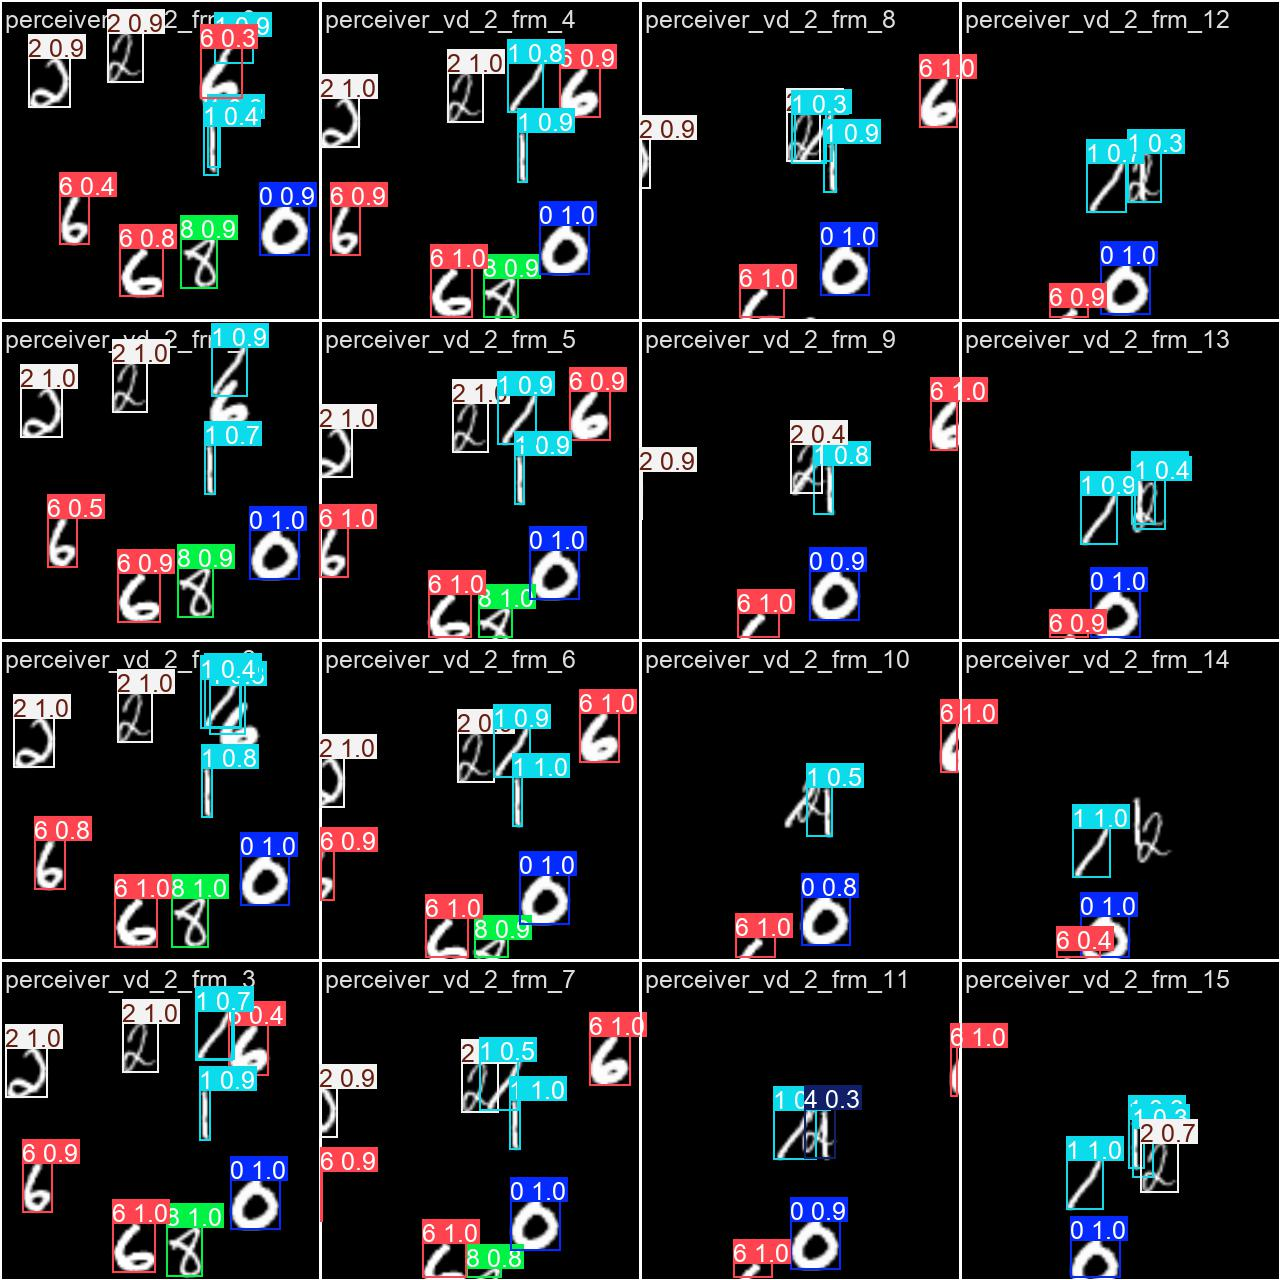
\includegraphics[width=\textwidth]{figures/figure_methods_val_batch2_pred_recurrent_perceiver.jpg}
    \caption{Visualization of RPerceiver predictions across sequential frames. Bounding boxes and confidence scores are displayed for detected digits. Notably, confidence scores can be less than 1.0 even for clear objects (e.g. digits in frame 1). Two challenging scenarios are analyzed: overlapping digits and digits near the frame border. The model shows limitations such as exhibiting false negatives with overlapping digits, as illustrated by the central cluster involving digits such as '1's and a '2' between frames 8 and 15. In contrast, predictions appear consistent between frames 5 and 13 for several digits near frame borders: the '2' and '6' on the left border, the '6' and '8' near the bottom border, and the '6' on the right border.}
    \label{fig:figure_methods_val_batch2_pred_recurrent_perceiver}
\end{figure}

\begin{figure}
    \centering
    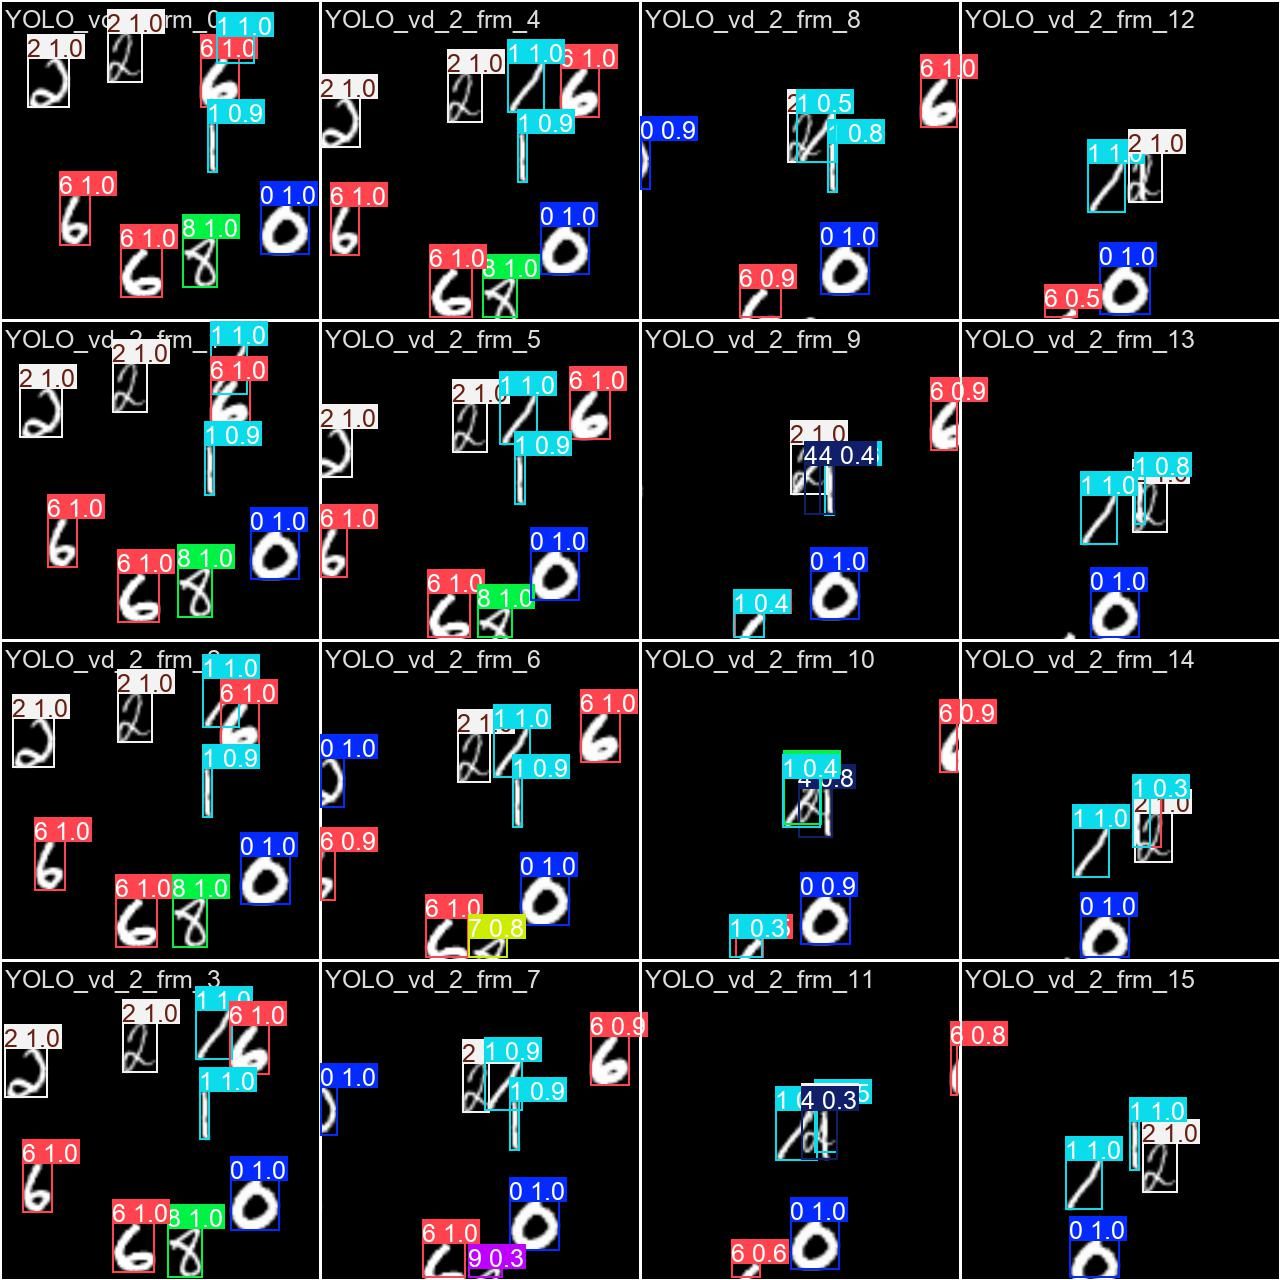
\includegraphics[width=\textwidth]{figures/figure_methods_val_batch2_pred_YOLO.jpg}
    \caption{Visualization of YOLOv8n \cite{Jocher_Ultralytics_YOLO_2023} predictions across sequential frames. Bounding boxes and confidence scores are displayed for detected digits. Notably, confidence scores are typically high (often 1.0) for relatively clear objects (e.g., digits in frame 1). Two challenging scenarios are analyzed: overlapping digits and digits near the frame border. The model appears to handle overlapping digits relatively effectively, with a few false negatives in the central cluster involving digits such as '1's and a '2' between frames 8 and 15. In contrast, predictions appear inconsistent between frames 5 and 13 for several digits near frame borders: the '2' on the left border, the '6' and '8' near the bottom border.}
    \label{fig:figure_methods_val_batch2_pred_YOLO}
\end{figure}

% TODO: recompute with tighter IoU threshold

To quantify the observations regarding model performance in challenging scenarios, as illustrated in Figures \ref{fig:figure_methods_val_batch2_pred_recurrent_perceiver} and \ref{fig:figure_methods_val_batch2_pred_YOLO}, we specifically evaluated the models on filtered subsets of the ground truth data. These subsets isolate two challenging conditions: overlapping objects (defined as pairs of ground truth objects with an Intersection over Union (IoU) greater than 0.01) and border objects (defined as ground truth objects whose bounding boxes intersect with the frame border). The resulting performance metrics for these specific cases are presented in Table \ref{tab:model_comparison_detailed}.

% YOLO:
% Raw Overlap mAP Results (Evaluator): {'map': tensor(0.8266), 'map_50': tensor(0.9133), 'map_75': tensor(0.8788), 'map_small': tensor(0.8266), 'map_medium': tensor(-1.), 'map_large': tensor(-1.), 'mar_1': tensor(0.7744), 'mar_10': tensor(0.8536), 'mar_100': tensor(0.8536), 'mar_small': tensor(0.8536), 'mar_medium': tensor(-1.), 'mar_large': tensor(-1.), 'map_per_class': tensor(-1.), 'mar_100_per_class': tensor(-1.), 'classes': tensor([0, 1, 2, 3, 4, 5, 6, 7, 8, 9], dtype=torch.int32)}

% Raw Boundary mAP Results (Evaluator): {'map': tensor(0.6989), 'map_50': tensor(0.7667), 'map_75': tensor(0.7365), 'map_small': tensor(0.6989), 'map_medium': tensor(-1.), 'map_large': tensor(-1.), 'mar_1': tensor(0.7119), 'mar_10': tensor(0.7280), 'mar_100': tensor(0.7280), 'mar_small': tensor(0.7280), 'mar_medium': tensor(-1.), 'mar_large': tensor(-1.), 'map_per_class': tensor(-1.), 'mar_100_per_class': tensor(-1.), 'classes': tensor([0, 1, 2, 3, 4, 5, 6, 7, 8, 9], dtype=torch.int32)}

% RPerceiver
% Raw Overlap mAP Results (Evaluator): {'map': tensor(0.6940), 'map_50': tensor(0.8853), 'map_75': tensor(0.7777), 'map_small': tensor(0.6940), 'map_medium': tensor(-1.), 'map_large': tensor(-1.), 'mar_1': tensor(0.6686), 'mar_10': tensor(0.7389), 'mar_100': tensor(0.7389), 'mar_small': tensor(0.7389), 'mar_medium': tensor(-1.), 'mar_large': tensor(-1.), 'map_per_class': tensor(-1.), 'mar_100_per_class': tensor(-1.), 'classes': tensor([0, 1, 2, 3, 4, 5, 6, 7, 8, 9], dtype=torch.int32)}

% Raw Boundary mAP Results (Evaluator): {'map': tensor(0.8470), 'map_50': tensor(0.9552), 'map_75': tensor(0.9101), 'map_small': tensor(0.8470), 'map_medium': tensor(-1.), 'map_large': tensor(-1.), 'mar_1': tensor(0.8512), 'mar_10': tensor(0.8739), 'mar_100': tensor(0.8739), 'mar_small': tensor(0.8739), 'mar_medium': tensor(-1.), 'mar_large': tensor(-1.), 'map_per_class': tensor(-1.), 'mar_100_per_class': tensor(-1.), 'classes': tensor([0, 1, 2, 3, 4, 5, 6, 7, 8, 9], dtype=torch.int32)}


\begin{table}[htb!]
    \centering
    \caption{Comparative analysis of YOLOv8n \cite{Jocher_Ultralytics_YOLO_2023} and RPerceiver on specific scenarios within the detection-moving-mnist-easy test split: object overlaps ('Overlap') and proximity to image borders ('Border'). Postprocessing ('Post') is applied to both models. The data indicates that the still-image detector YOLOv8n achieves higher accuracy on overlapping objects. In contrast, RPerceiver significantly outperforms YOLOv8n on border cases, supporting the hypothesis that it effectively leverages temporal information from the video sequence.}
\label{tab:model_comparison_detailed}

    \label{tab:model_comparison_detailed}
    \begin{tblr}{width=1\textwidth, hlines, vlines,
                  colspec = { l c c c c c },
                  row{1} = {font=\bfseries},
                 }
        \SetCell[r=2]{l}Model & \SetCell[r=2]{l}Post & \SetCell[c=3]{c}Overlap & & & \SetCell[c=3]{c}Border & & \\
                   &   & mAP_{50} & mAP_{75}  & mAP_{50-95}       & mAP_{50} & mAP_{75}  & mAP_{50-95}  \\
        YOLOv8n    & X & \textbf{91.3}  & \textbf{87.9} & \textbf{82.7} & 76.7  & 73.7 & 69.9 \\
        RPerceiver & X & 88.5 & 77.8 & 69.4  & \textbf{95.5} & \textbf{91.0} & \textbf{84.7}\\
    \end{tblr}
\end{table}

\subsection{Ablation Study} \label{Experiments:AblationStudy}

We evaluate how is robustness the RPercevier and RPerceiverMM against sensor complete failure or non-detemenistic input of sensor input. We run use center point prediction task. We experimented with two setup configurations: \texttt{single-view} and \texttt{multi-view}. First, the single-view configuration used a single camera sensor, representing the most basic object detection task for video input. Second, we used a multi-view camera setting where the model processed information from different cameras to perform object detection within a unified spatial representation generated from these inputs.

We considered three distinct evaluation procedures: \texttt{default}, \texttt{shuffle}, and \texttt{blind}. Additionally, we evaluated a combination of the last two.

\begin{description}
    \item[\texttt{default}] This procedure represents the normal operational regime where all sensors function as expected.

    \item[\texttt{shuffle}] In this procedure, the sensor inputs are randomly permuted within each time step. Consequently, the model receives inputs from the sensors in a random order for that specific time step. Shuffling only occurs for the sensors inputs within the same time step. This procedure is only applicable to a multi-view setup.

    \item[\texttt{blind}] This procedure simulates a sensor failure mode where the input from one or more camera sensors is unavailable. The \texttt{blind} evaluation procedure is implemented by dropping the input stream from the affected sensor(s) after a midpoint time step $t_{half}$. Therefore, information from sensor(s) for the second half of the sequence becomes unavailable to the model. 
\end{description}

% TODO: Explain relevance of dropout and blind


Table~\ref{tab:results_single_view_default} shows the inference results for single-view setup under default evaluation procedure. We compare models under two training procedures. 

We ran a "default" evaluation where none of the frames were dropped. We evaluated the performance separately for each different number of digits per video sequence. 
\begin{table}[htb!]
    \centering
    \caption{Results for single-view the "default" evaluation where none of the frames were dropped. (d) next to the model name indicates a training procedure with frame dropout. Results are broken down by the number of digits in the frame. The Average Displacement Error (ADE) measures the error for the second half of the sequence. The Final Displacement Error (FDE) evaluates the error for the last frame in the sequence.}
    \label{tab:results_single_view_default}
    \begin{tblr}{width=1\textwidth, hlines, vlines,
                    colspec = { l c c c c c c c c c c },
                    row{1} = {font=\bfseries},
                    row{2} = {font=\bfseries},
                }
        \SetCell[r=2]{l} Model & \SetCell[c=2]{c}1 digit & & \SetCell[c=2]{c}2 digits & & \SetCell[c=2]{c}4 digits & & \SetCell[c=2]{c}8 digits & & \SetCell[c=2]{c}10 digits & \\
        & ADE & FDE & ADE & FDE & ADE & FDE & ADE & FDE & ADE & FDE \\
        RP              & \textbf{0.717} & \textbf{0.725} & \textbf{0.794} & \textbf{0.793} & \textbf{0.958} & \textbf{0.934} & \textbf{1.520} & \textbf{1.382} & \textbf{3.273} & \textbf{2.611} \\
        RP (d) & 0.745 & 0.793 & 0.838 & 0.882 & 1.034 & 1.065 & 1.656 & 1.583 & 3.626 & 3.12 \\
    \end{tblr}
\end{table}

We conducted a "blind" evaluation where the second half of the sequence was dropped. Table~\ref{tab:results_frame_dropout_blind} shows the results. We observed an increase in error metrics for the model trained without frame drops. Conversely, the model trained with frame drops maintains low errors.

\begin{table}[htb!]
    \centering
    \caption{Results for the "blind" evaluation where the second half of the sequences is dropped. (d) next to the model name indicates a training procedure with frame drops. Results are broken down by the number of digits in the frame. The Average Displacement Error (ADE) measures the error for the second half of the sequence. The Final Displacement Error (FDE) evaluates the error for the last frame in the sequence.}
    \label{tab:results_frame_dropout_blind}
    \begin{tblr}{width=1\textwidth, hlines, vlines,
                    colspec = { l c c c c c c c c c c },
                    row{1} = {font=\bfseries},
                    row{2} = {font=\bfseries},
                    colsep=3pt, % Reduced column separation
                }
        \SetCell[r=2]{l} Model & \SetCell[c=2]{c}1 digit & & \SetCell[c=2]{c}2 digits & & \SetCell[c=2]{c}4 digits & & \SetCell[c=2]{c}8 digits & & \SetCell[c=2]{c}10 digits & \\
        & ADE & FDE & ADE & FDE & ADE & FDE & ADE & FDE & ADE & FDE \\
        RP              & 42.210 & 34.754 & 36.087 & 28.83014 & 32.146 & 24.397 & 31.32972 & 23.730 & 33.334 & 25.935 \\
        RP (d)             & \textbf{1.541} & \textbf{1.101} & \textbf{1.907} & \textbf{1.364} & \textbf{2.658} & \textbf{1.905} & \textbf{5.084} & \textbf{3.679} & \textbf{8.198} & \textbf{6.627} \\
    \end{tblr}
\end{table}


For the purpose of some of the experiment we additionally divide the frame into grid views. In this way we mimic a Bird Eye View (BEV) (see Figure~\ref{fig:figure_methods_dataset_image_view_bev}).

\begin{figure}
    \centering
    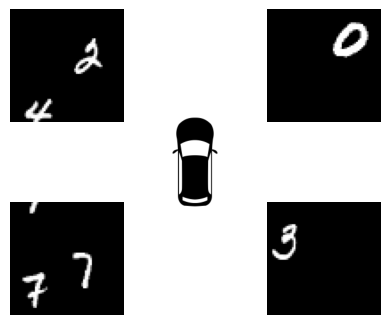
\includegraphics[width=0.33\textwidth]{figures/figure_methods_dataset_image_view_bev.png}
    \caption{Bird Eye View (BEV) of the frame raster divided into grid.}
    \label{fig:figure_methods_dataset_image_view_bev}
\end{figure}

Table~\ref{tab:results_multi_view} shows the inference results for multi-view setup we breakdown reasults by evaluation procedure. We train models under training schemas. 

% Results: https://docs.google.com/spreadsheets/d/1shITm2iWIKzAAlWpRwED-g1H6YurMJoJgxagRU2x6Gg/edit?gid=290835343#gid=290835343
% TODO Consider to reduce width of the table

\begin{table}[htb!]
    \centering
    \caption{Results for the "default" and "blind" experiments with sensor output shuffle. An asterisk (*) next to the model name indicates a training procedure with sensor output drops. The Average Displacement Error (ADE) measures the error for the second half of the sequence. The Final Displacement Error (FDE) evaluates the error for the last frame in the sequence.}
    \label{tab:results_multi_view}
    \begin{tblr}{
        hlines, vlines,
        colspec={l c c c c c c c c c},
        row{1}={font=\bfseries},
        row{2}={font=\bfseries},
    }
        \SetCell[r=2]{l}Model & \SetCell[c=2]{c}Default & & \SetCell[c=2]{c}Shuffle & & \SetCell[c=2]{c}Blind & & \SetCell[c=2]{c}Blind, Shuffle & & \SetCell[r=2]{l}{Params \\ (M)} \\
        & ADE & FDE & ADE & FDE & ADE & FDE & ADE & FDE &\\
        RPMM & 0.760 & 0.753 & 23.701 & 23.759 & 17.952 & 25.568 & 25.559 & 24.696 & 1.2 \\
        RPMM (s) & 0.823 & 0.814 & 0.812 & 0.799 & 13.644 & 20.124 & 13.670 & 20.080 & 1.2 \\
        RPMM (d) & 0.881 & 0.937 & 4.043 & 4.345 & 1.471 & 2.093 & 5.648 & 7.341 & 1.2 \\
        RPMM (d, s) & 1.073 & 1.152 & 0.956 & 1.022 & 1.729 & 2.345 & 1.632 & 2.287 & 1.2 \\
    \end{tblr}
\end{table}


% \section{Text Creation} \label{textCreation}
By the time You start using this template, You have likely completed its contents using a more comfortable and collaborative software like Google Docs. Starting formatting makes sense only when the contents of Your work no longer change much. Otherwise, the changes in the content may require doing the formatting part again. Still, some formatting-related recommendations are relevant a lot earlier than when formatting the draft to a fair copy.

\subsection{Chapters}
Your thesis chapters should be evenly balanced with each other. Because this template focuses on formatting, then that guideline is broken here (the previous chapter~\ref{formatting} is noticeably lengthier than this chapter~\ref{textCreation}). In Your work, all the chapters besides the Introduction and Conclusion should have a relatively even length. This principle also helps You not overdo a single part of Your work but spread Your attention to all the essential parts. What precisely these parts are depends on Your thesis type. The University of Tartu’s Institute of Computer Science’s thesis preparation and grading guidelines document defines a certain number of these types. The study or research group where You are doing Your thesis might define continuations of those types. Ensure that Your thesis document provides a balanced coverage of all Your chosen thesis type requires.

\begin{wrapfigure}{r}{0.33\textwidth}
    \centering
    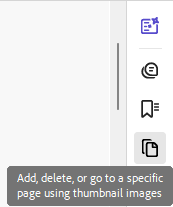
\includegraphics[width=0.33\textwidth]{figures/Figure5-AcrobatReaderMenu.png}
    \caption{The right-hand menu of Acrobat Reader.}
    \label{fig:acrobatReaderMenu}
\end{wrapfigure}
By the time Your thesis starts to take shape, it is useful to look at Your document as a whole. This can be done, for example, with the page order changing tool (\emph{Add, delete, or go to specific page using thumbnail images}) in the Acrobat Reader PDF viewer. The view from that tool shows You Your thesis as a whole. Just like if You would have printed out all of the pages and spread them across a desk. From that view, You see if all the different parts of the document are balanced and in visual equilibrium (see Figure~\ref{fig:acrobatReaderOverview}).

Seda saab teha näiteks Acrobat Reader PDF vaaturis lehekülgede järjekorra muutmise (\emph{Add, delete, or go to specific page using thumbnail images}) tööriistaga (vt joonis~\ref{fig:acrobatReaderMenu}). Tolle tööriista kuva näitab Teile tervet Teie tööd ülevaatlikult. Justkui oleksite oma töö välja printinud ja kõik lehed eraldi suure laua peale laotanud. Sellest ülevaatest Te näete, kas Teie erinevad töö osad on omavahel tasakaalus ja visuaalselt kooskõlas (vt joonis~\ref{fig:acrobatReaderOverview}).

\begin{figure}[t]
    \centering
    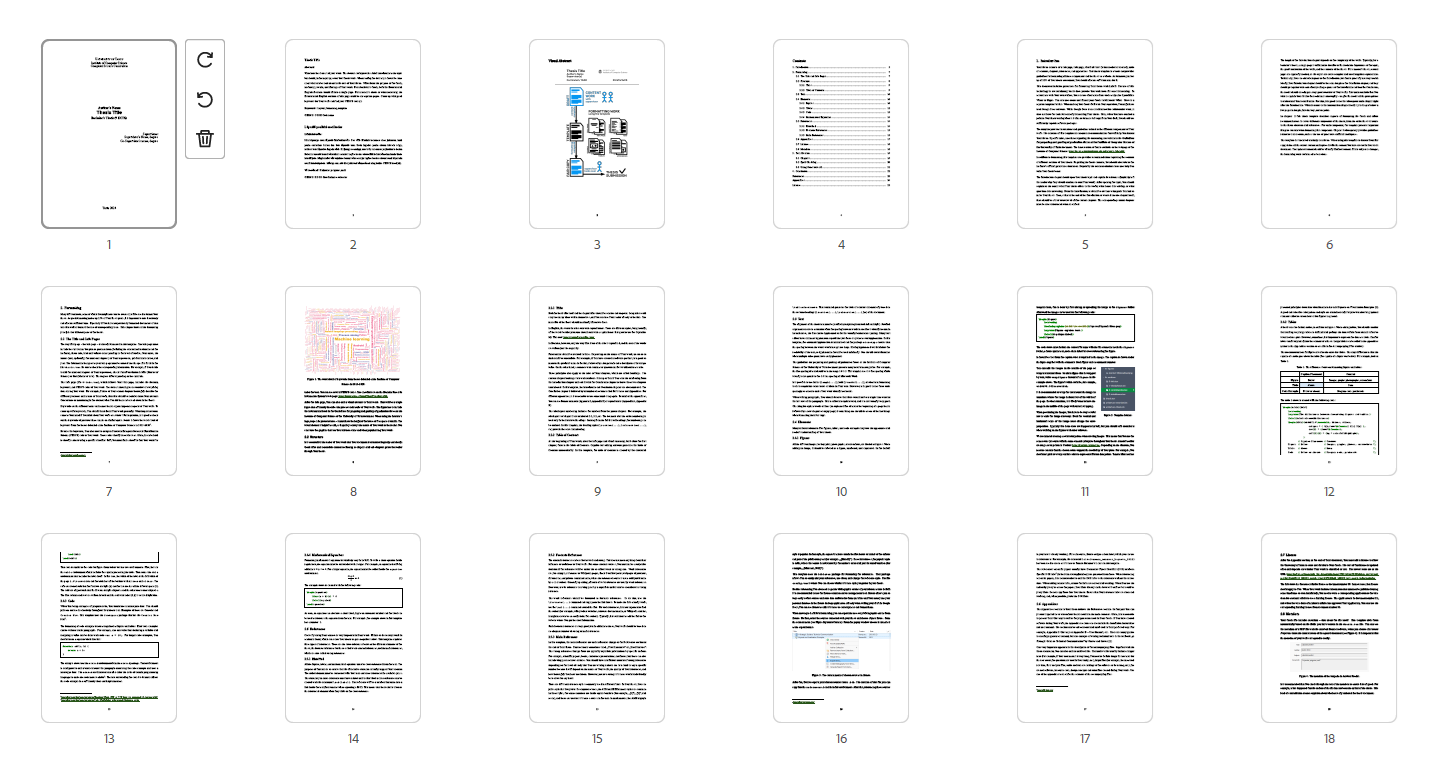
\includegraphics[width=\textwidth]{figures/Figure6-AcrobatReaderOverview.png}
    \caption{The overview of the thesis template in Acrobat Reader.}
    \label{fig:acrobatReaderOverview}
\end{figure}
he birds-eye view of the thesis also shows You if all the necessary places have text. For example, every chapter should start with a brief introductory text. This text must be after the   heading and before any subheadings. That introductory text usually explains why the corresponding chapter is necessary for Your work and what the reader can expect from the subchapters. In addition to that, the (sub)chapters could be woven together with connective sentences, and every bigger chapter could end with a conclusive paragraph. No chapter should start or end with any elements (figures, tables, code examples, equations) or a list. Your thesis text must be smooth to read.

\subsection{Spell Checking}
Microsoft Word’s speller, which You should turn on, comes in really handy when formatting Your fair copy. Having worked on Your draft a lot, You might have gotten used to looking at the same text over and over again; thus, noticing spelling mistakes Yourself might be quite difficult. There are spelling and proofing tools in Word for both the Estonian and English languages. Presenting a thesis that has grammatical errors can result in a lower grade.

Of course, You are also free to use tools that provide grammatical assistance, such as Grammarly, if You have access to such tools, and they make Your work more effective.

\subsection{Using Generative AI}
Using generative AI tools can also make Your work more effective. Here, their use for purely text editing purposes is focused on. When You have also used generative AI for content-related purposes (for example, to create Your questionnaire questions), You should definitely detail Your generative AI usage within the contents of Your thesis text. However, using it for editing Your thesis text is not content-related, so it will suffice to mention its use at the end of the Introduction chapter.

One good way to use a generative AI chatbot is to give it a paragraph of Your text and a prompt to make the specified academic text more readable. When doing that, You should read the result and correct it as needed. The AI chatbot might have mutated Your thoughts in the text, and You must restore them. Also, You might not personally agree with the specific style that AI has provided You and may want to keep tweaking it. The generative AI tools can very effectively help improve Your text flow, but You have to be very keen to ensure that the modified text still conveys Your thoughts and that You agree with the proposed writing style.

It is certainly not effective to use paragraphs that are solely generated by AI in Your thesis text. The author of the thesis is still You. This means that You are responsible for what is written in Your document. Typically, the text written by AI tends to be too general, overly illustrative and includes factual errors that a knowledgeable human author would not make. You do not want to put Yourself into a situation where You have to direct blame towards an AI chatbot due to issues in Your thesis text.

\section{Conclusion} \label{Conclusion}

Two novel architectures were introduced: the Recurrent Perceiver (RPerceiver) and its multi-modal variant (RPerceiverMM). These were inspired by the Perceiver architecture's \cite{jaeglePerceiverGeneralPerception2021} ability to handle high-dimensional, multi-modal data but were adapted for sequential inputs, such as video. To facilitate this research, a novel dataset, "detection-moving-mnist-easy", was generated. This dataset provides controlled video sequences with annotations for evaluating both bounding box and center point (keypoint) prediction tasks.

The RPerceiver was compared against a strong baseline, YOLOv8n \cite{Jocher_Ultralytics_YOLO_2023}, on the bounding box detection task.
While both models showed similar $mAP@0.5$ and $mAP@0.75$ scores, YOLOv8n performed better at $mAP@0.5:0.95$. Further evaluation showed that YOLOv8n performed better with overlapping objects when the $\mathrm{IoU}$ between objects was $\gt 10\%$. However, the RPerceiver demonstrated superior performance in handling objects near frame borders, suggesting its effectiveness in leveraging temporal information, particularly when objects have partial visibility.
Notably, RPerceiver achieved competitive mAP scores with significantly fewer parameters and lower computational cost compared to YOLOv8n.

Another contribution of this work was the investigation of training strategies to enhance model resilience against sensor input degradation, simulating real-world Autonomous Driving Systems (ADS) challenges like complete sensor failure and asynchronous data arrival.
\texttt{dropout} and \texttt{shuffle} training procedures were introduced and evaluated.
Ablation studies using the center point prediction task demonstrated the efficacy of these strategies. In single-view scenarios, training RPerceiver with \texttt{dropout} resulted in significantly better performance under simulated complete sensor failure compared to the baseline model, although it incurred a minor performance penalty under normal conditions.

Extending the analysis to multi-view scenarios using RPerceiverMM, the benefits of targeted training procedures were further confirmed. Models trained with input \texttt{shuffling} excelled when evaluated with shuffled sensor inputs, while \texttt{dropout}-trained models showed the best robustness against simulated sensor failure.
The model trained with both \texttt{dropout} and \texttt{shuffling} provided the most robust performance under the combined \texttt{blind, shuffle} evaluation, highlighting the potential for tailoring training methods to specific anticipated failure modes.
While these robustness-enhancing training procedures introduced a slight performance decrease under default, non-degraded conditions, they offer substantial improvements in resilience against common sensor issues faced by ADS.


\clearpage
\printbibliography[heading=bibintoc]

\section*{Appendices} \label{appendices} \addcontentsline{toc}{section}{Appendices}

\subsection*{A. Training Hyperparameters} \label{Appendix:TrainingHyperparameters}

\begin{table}[htb!]
    \centering
    \caption{Hyperparameters used for training the RPerceiver model for bounding box prediction task.}
    \label{tab:training_params_bbox_20250505}
    \begin{tblr}{width=1\textwidth, hlines, vlines,
                   colspec = { l l X },
                   row{1} = {font=\bfseries},
                   colsep=3pt,
                  }
        Hyperparameter & Value & Description \\
        backbone & cnn & Backbone type \\
        batch\_size & 1 & Batch size for training \\
        bbox\_loss\_coef & 5 & L1 box coefficient \\
        eos\_coef & 0.1 & Relative classification weight of the no-object class \\
        epochs & 32 & Number of training epochs \\
        giou\_loss\_coef & 2 & GIoU box coefficient \\
        learning\_rate & 0.0001 & Learning rate \\
        learning\_rate\_backbone & 0.0001 & Learning rate \\
        num\_frames & 20 & Number of frames. \\
        object\_detection & True & Use object detection prediction head \\
        resize\_frame & 320 & Resize frame to this size \\
        scheduler\_step\_size & 18,28 & Scheduler step size \\
        set\_cost\_bbox & 5 & L1 box coefficient in the matching cost \\
        set\_cost\_class & 1 & Class coefficient in the matching cost \\
        set\_cost\_giou & 2 & giou box coefficient in the matching cost \\
        weight\_decay & 0.01 & Weight decay for optimizer \\
        weight\_loss\_bce & 1 & Weight loss binary cross entropy \\
        weight\_loss\_center\_point & 5 & Weight loss center point \\
    \end{tblr}
\end{table}

\begin{table}[htb!]
    \centering
    \caption{Hyperparameters used for training the RPerceiverMM model for center point task.}
    \label{tab:training_params_cp_20250505}
    \begin{tblr}{width=1\textwidth, hlines, vlines,
                   colspec = { l l X },
                   row{1} = {font=\bfseries},
                   colsep=3pt,
                  }
        Hyperparameter & Value & Description \\
        backbone & cnn & Backbone type \\
        batch\_size & 1 & Batch size for training \\
        bbox\_loss\_coef & None & L1 box coefficient \\
        eos\_coef & None & Relative classification weight of the no-object class \\
        epochs & 21 & Number of training epochs \\
        giou\_loss\_coef & None & GIoU box coefficient \\
        learning\_rate & 0.0001 & Learning rate \\
        learning\_rate\_backbone & 0.0001 & Learning rate \\
        num\_frames & 12 & Number of frames. \\
        object\_detection & None & Use object detection prediction head \\
        resize\_frame & None & Resize frame to this size \\
        scheduler\_step\_size & 18 & Scheduler step size \\
        set\_cost\_bbox & None & L1 box coefficient in the matching cost \\
        set\_cost\_class & None & Class coefficient in the matching cost \\
        set\_cost\_giou & None & giou box coefficient in the matching cost \\
        weight\_decay & 0.01 & Weight decay for optimizer \\
        weight\_loss\_bce & 1 & Weight loss binary cross entropy \\
        weight\_loss\_center\_point & 5 & Weight loss center point \\
    \end{tblr}
\end{table}

\clearpage
\subsection*{B. Model Hyperparameters} \label{Appendix:ModelHyperparameters}

\begin{table}[htb!]
    \centering
    \caption{Hyperparameters used for configuring RPerceiver model.}
    \label{tab:model_params_RPerceiver_20250505}
    \begin{tblr}{width=1\textwidth, hlines, vlines,
                   colspec = { l l X },
                   row{1} = {font=\bfseries},
                   colsep=3pt,
                  }
        Hyperparameter & Value & Description \\
        enc\_layers & 1 & Number of layers in Perceiver encoder \\
        enc\_nheads\_cross & 1 & Number of cross-attention heads \\
        hidden\_dim & 128 & Latent dimension size \\
        max\_freq & 10 & Maximum frequency for Fourier encoding \\
        nheads & 1 & Number of latent self-attention heads \\
        num\_freq\_bands & 6 & Number of frequency bands for Fourier encoding \\
        num\_queries & 16 & Number of latents, or induced set points, or centroids \\
        self\_per\_cross\_attn & 1 & Number of self-attention blocks per cross-attention block \\
    \end{tblr}
\end{table}

\begin{table}[htb!]
    \centering
    \caption{Hyperparameters used for configuring RPerceiverMM model.}
    \label{tab:model_params_RPerceiverMM_20250505}
    \begin{tblr}{width=1\textwidth, hlines, vlines,
                   colspec = { l l X },
                   row{1} = {font=\bfseries},
                   colsep=3pt,
                  }
        Hyperparameter & Value & Description \\
        enc\_layers & 1 & Number of layers in Perceiver encoder \\
        enc\_nheads\_cross & 1 & Number of cross-attention heads \\
        hidden\_dim & 128 & Latent dimension size \\
        max\_freq & 10 & Maximum frequency for Fourier encoding \\
        nheads & 1 & Number of latent self-attention heads \\
        num\_freq\_bands & 6 & Number of frequency bands for Fourier encoding \\
        num\_queries & 16 & Number of latents, or induced set points, or centroids \\
        self\_per\_cross\_attn & 1 & Number of self-attention blocks per cross-attention block \\
    \end{tblr}
\end{table}

\section*{License} \label{license} \addcontentsline{toc}{section}{License}
To here You must add a license that allows the University of Tartu to store and publish Your thesis. The newest license texts can be found at the following address:

\url{https://adr.ut.ee/?page=pub_list_dynobj&desktop=57835&tid=70993&data_only=true&search=Otsi&field_100193_search_type=ANY&field_100193_text_search_value=ppimine}

Please read chapter~\ref{subchapter:license} in this template to know what license You have to use on this page.


\end{document}



